\documentclass[a4paper,12pt]{book}
\usepackage[utf8]{inputenc}
\usepackage{amsmath,amssymb,latexsym}
\usepackage{graphicx,subfigure}
\usepackage{tcolorbox}
\usepackage{wrapfig}
\usepackage{rotating}
\usepackage[margin=2.5cm]{geometry}
\newtheorem{Equation}{\indent Equation}[section]
\textwidth=6in
\renewcommand{\baselinestretch}{1.5}

\begin{document}

\author{Zachary Matheson}
\title{Fission in Exotic Nuclei Using DFT}
\date{Revised May 2018}

\frontmatter
\maketitle
\tableofcontents

\mainmatter
\chapter{Introduction}\label{chap:Intro}

\section{History of fission theory}
Nuclear fission is the fundamental physical process by which a heavy nucleus decays into two smaller nuclei of comparable masses, and a proper understanding of fission is critical for applications in reactor physics, nuclear astrophysics, and stockpile stewardship. Fission was first observed by Hahn and Stra\ss{}mann in 1939~\cite{Hahn1939} when they bombarded uranium atoms with neutrons and detected barium, a paradoxically lighter element, but at the time they were unable to explain their observations. An explanation came shortly thereafter in letters to Nature by Meitner and Frisch~\cite{Meitner1939b} and by Bohr~\cite{Bohr1939a}. Meitner and Frisch's described the findings in the following way:

\begin{quote}
On account of their close packing and strong energy exchange, the particles in a heavy nucleus would be expected to move in a collective way which has some resemblance to the movement of a liquid drop. If the movement is made sufficiently violent by adding energy, such a drop may divide itself into two smaller drops\dots \ It seems therefore possible that the uranium nucleus has only small stability of form, and may, after neutron capture, divide itself into two nuclei of roughly equal size (the precise ratio of sizes depending on finer structural features and perhaps partly on chance).
\end{quote}

\noindent In addition to neutron-induced fission, spontaneous fission, which is a different form of fission so-dubbed because it occurs without bombardment by neutrons or any other projectiles, was reported by Flerov and Petrjak in a single-paragraph letter to \textit{Physical Review} in 1940~\cite{Flerov1940}. For the remainder of this dissertation, I will be referring mainly to spontaneous fission unless stated otherwise.

%It is a highly-collective process involving all the constituent nucleons of the system, and thus since its discovery, it has been described via large shape deformations of an otherwise spherical (or nearly-spherical) ``drop'' of nucleons~\cite{Bohr1939}. 

Following the explanation of Meitner and Frisch, fission is relatively simple to conceptualize, but remarkably difficult to explain quantitatively. Quantitative fission predictions based on fundamental nuclear theory are challenging because of the large number of particles involved, along with the complex collective interactions which take place when one system deforms and becomes two. Historically, one could argue that theoretical attempts to describe nuclear fission have leapt forward in three major waves.

\subsection{Liquid drop model}
The first major wave in nuclear fission theory goes back to the very beginning of the nuclear age in the 1930s with the liquid drop model. The liquid drop model was first developed by Weizs\"acker in 1935~\cite{Weizsacker1935} as a way to describe collective properties of nuclei. It was later adapted by Bohr and Wheeler to quantitatively describe nuclear fission in terms of bulk properties of nuclei~\cite{Bohr1939}. This model was able to successfully describe nuclear binding energies and the energetics of nuclear fission.

The liquid drop model has its weaknesses, however. For example, it could not explain the fission fragment mass asymmetry which characterizes spontaneous fission in many actinides. Furthermore, until the 1960s, nuclear fission was treated as though separate from the rest of nuclear physics, with little attention given to the quantum nature of its constituent particles.%.. See the first few paragraphs of~\cite{Grant1976} for more of this story.

\subsection{Microscopic-macroscopic approach}
The second theoretical wave came during a time of renewed interest in fission, triggered by the discovery of fission isomerism in 1962 by Polikanov, et al~\cite{Polikanov1962}. This was understood as a manifestation of nuclear shape deformation based on a prediction by Nilsson~\cite{Nilsson1955}. Recognizing the important connection between shell effects, collective shape deformations, and the fission process, Strutinsky added a quantum mechanical correction to the liquid drop energy in 1967 in order to account for the added stability that occurs when a nucleus contains a ``magic number'' of protons and/or neutrons~\cite{Strutinsky1967, Strutinsky1968, Brack1972}. These models go by the name ``microscopic-macroscopic'' because they combine the ``macroscopic'' bulk properties of the liquid-drop model with the ``microscopic'' quantum mechanical Strutinsky shell correction.

Microscopic-macroscopic (``micmac'') fission models are computationally inexpensive, and can achieve quite satisfactory results (some recent highlights from the Los Alamos and Warsaw groups include Refs.~\cite{Moller2015a,Moller2015b,Jachimowicz2013,Jachimowicz2017}). In this approach, for instance, the mysterious fragment mass asymmetry that occurs in actinides is understood to be a manifestation of strong shell effects within the fragments during the split. However, since the model is based on a phenomenological description of what is actually a quantum many-body system, its predictive power is limited, with no clear way of making systematic improvements. Micmac models also rely on many parameters which must be fit to data, and are therefore subject to all the dangers that come with parameter fitting. A more fundamental approach would be to consider many individual nucleon states using a quantum many-body method. 

\subsection{Self-consistent models and the supercomputing era}
The third major wave is taking place now, heralded by the age of supercomputers. In fact, fission was listed as an exascale problem in a 2017 technical report to the Department of Energy~\cite{Carlson2017} - that is, one of the problems which motivates the drive towards exascale computing. For large systems with many, many particles, density functional theory (DFT) is a way to recast the ${\sim}$200 particle Schr\"{o}dinger equation into a simpler problem involving only a few densities and currents (see Section~\ref{sect:DFT} as well as~\cite{bender2003}). State-of-the-art calculations such as the ones described in this dissertation and others reviewed in~\cite{schunck2016} allow us to combine nuclear DFT techniques with modern high-performance computing platforms to predict fission properties, such as lifetimes and fragment yields.% Many of the ideas which are used today were inspired by previous work done with the liquid drop and micmac models. The approach used throughout this dissertation is described in Chapter~\ref{chap:Model}.

These advances in computing come simultaneously with technological advances which allow experimental nuclear physics to reach far beyond what has been achieved previously. New facilities include the Facility for Rare Isotope Beams (FRIB) at Michigan State University, which is projected to nearly double the number of isotopes which can be produced synthetically~\cite{Baumann2016}, and the Superheavy Elements Factory in Dubna, Russia~\cite{dmitriev2016}, which focuses on the synthesis of new superheavy elements and detailed study of superheavy isotopes that have already been created. Other, existing facilities have received, or will soon receive, upgrades which should allow them to produce experimental fission data that is much more detailed and precise than ever before~\cite{Andreyev2018}. Together, state-of-the-art facilities for experiment and high-performance computing for theory are expected to lead to rapid advancement in our understanding of atomic nuclei and their decays.

\section{The scope of this dissertation}
Microscopic models (as self-consistent models are often called) are increasingly able to predict properties of fission fragments; however, a comprehensive microscopic description of fission fragments (including mass and charge distributions, excitation and kinetic energy distributions, angular dependence, spin, neutron emission) remains elusive. Chapter~\ref{chap:Model} will discuss our approach for estimating the mass and charge of fission fragments.

%Additionally, static models are not well-suited to describing the process of a single nucleus becoming two, an inherently time-dependent process. How can one precisely identify two distinct fragments when the wavefunctions of one fragment’s constituent nucleons may extend into the opposite fragment? How do correlations between nucleons affect the energetics of the resulting fragments? A better understanding of the mechanism of fragment formation can help guide and refine fission fragment models. This will be discussed in Section~\ref{sect:loc-frags}.

The next challenge is to do these calculations cheaply. In every theoretical calculation, one must ask the questions ``What approximations can I safely make?'' and ``What are the important degrees of freedom for this problem, and which can I ignore?'' These simplifications, together with improvements to the computational workflow itself, such as better file handling and parallelization, can significantly reduce the total time-to-answer. Computational details will be discussed in Chapter~\ref{chap:Numerical}.

After describing the model in Chapters~\ref{chap:Model} and~\ref{chap:Numerical}, it is applied to several isotopes in Chapters~\ref{chap:178Pt}-~\ref{chap:rprocess} to compute primary fragment yields. Historically, most experimental and theoretical studies of fission have centered around the region of actinides near $^{235}$U, which includes isotopes of uranium, plutonium, and thorium relevant for reactor physics and stockpile stewardship. Isotopes in this region tend to fission asymmetrically, with the larger prefragment influenced by the doubly-magic shell structure of $^{132}$Sn and resulting in a heavy fragment distribution centered around ${\sim}^{140}$Te. However, given the aforementioned recent interest in rare and exotic nuclei, we have applied our model to study fragment distributions in exotic systems found in other regions of the nuclear chart. First, in Chapter~\ref{chap:178Pt} we discuss bimodal fission in the neutron-deficient isotope {\Pt}, which until recently was conventionally expected to fission symmetrically. This region is a good one in which to test fission models because of the large isospin asymmetry ($N/Z\approx1.3$ in this region, compared to $N/Z\approx1.5$ near the valley of stability). Then in Chapter~\ref{chap:294Og} we discuss cluster radioactivity in {\Og}, the heaviest element ever produced in a laboratory. In Chapter~\ref{chap:rprocess} we move to the neutron-rich side of the nuclear chart ($N/Z>1.7$) to study isotopes which are expected to play a significant role in the astrophysical r process. %\textbf{Along the way, we will discuss some of the issues related to fragment identification and yield prediction.}

%The calculations in Chapters~\ref{chap:178Pt},~\ref{chap:294Og}, and~\ref{chap:rprocess} are relatively expensive. To perform large-scale exploratory studies in other regions of the nuclear chart, it will be necessary to find ways to reduce the total computational cost of these calculations. One method, still in its infancy, offers a promising approach for identifying fission fragment distributions using a significantly-reduced potential energy surface, which is by far the biggest bottleneck in our calculations. In Chapter~\ref{append:Fragments}, we discuss the problem of scission and present an alternative method for identifying fragments based on the nucleon localization function.

%Alternatively, at the end of each Chapter, we say a few words about challenges faced during the project and new physical insights gained that aren't related to the overall narrative of the Chapter, but which are nevertheless useful for future model developments.

This dissertation concludes in Chapter~\ref{chap:Outlook} with a discussion of our results and their significance. Suggestions are then made for future model developments, computational improvements, and physical applications.
 % Introduction
\chapter{Describing fission using nuclear density functional theory}\label{chap:Model}

%(Nicolas gave a good annotated presentation in 2017 that describes some of the philosophy, as well as some of the outstanding challenges of spontaneous fission in an adiabatic framework: \verb|https://t2.lanl.gov/fiesta2017/school/Schunck_NotesSlides.pdf|)

There are basically two microscopic frameworks in which to study fission: time-dependent and static (time-independent). Since fission is an inherently time-dependent process, time-dependent methods offer deep insight into the fission process and the characteristics of the fragments, especially kinetic and excitation energies~\cite{Scamps2019, Scamps2015a, Simenel2014, Bulgac2016a, Umar2010}. However, they can only treat a single event at a time and are quite expensive, making them impractical for fission yield predictions. Furthermore, and most important to a discussion of spontaneous fission, is the fact that fully time-dependent approaches have no mechanism with which to describe quantum tunneling, making them totally unsuited to spontaneous fission calculations. Finally, even if the tunneling problem was solved, this approach would still be unsuitable for any nucleus with a reasonably-long lifetime (compared to a typical time step size ${\sim}10^{-22}$ sec).

In the other, so-called static approach, it is assumed that collective motion of the nucleus is slow compared to the intrinsic motion of the nucleons, and therefore that collective and intrinsic degrees of freedom can be decoupled. This assumption of adiabaticity is supported by experimental evidence which suggests a characteristic timescale for fission (from saddle to scission, the point at which the neck snaps) of ${\sim}10^{-20}-10^{-18}$sec, compared to typical nuclear timescales on the order of ${\sim}10^{-22}$sec (see~\cite{Jacquet2009} for a review of fission timescale experiments). The validity of the adiabatic assumption was further discussed for fission and other nuclear processes in~\cite{Nazarewicz1993}.

The assumption of adiabaticity justifies the creation of a potential energy surface (PES) in some space of collective shape coordinates, and the dynamics of fission are then described in terms of trajectories across the PES. Quantum tunneling pops out in a fairly natural way in this formalism using the WKB approximation, and half-life estimates follow. The kinetic and excitation energies can be computed in this framework, but they are extremely sensitive to the characterization of scission, which is not well-defined in static frameworks~\cite{Younes2011}. However, as we shall show, the static approach is well-suited to estimating fission yields.

%Adiabaticity: For fusion reactions, N,Z equilibrium reached in ${\sim}10^{-21}$ seconds, then energy/thermal equilibrium in a similar time scale, then finally mass equilibrium in ${\sim}10^{-19}$ - Yuri has a slide with these time scales from his talk Monday. By comparison, what is an appropriate timescale for collective motion? I suppose that is nucleus-dependent

In an effort to be as self-consistent as possible, the PES is computed in the framework of nuclear DFT, which combines the Hartree-Fock-Bogoliubov variational approximation to the energy with a many-body method inspired by Kohn-Sham DFT. An overview of this self-consistent mean-field framework is described below, followed by a description of the dynamical calculations which are used to calculate fission yields.

\section{Nuclear density functional theory}
As with all nonrelativistic quantum systems, nuclei can be described using the many-body Schr\"{o}dinger equation. However, one often finds this type of description difficult or impossible in practice, for two reasons:

\begin{itemize}
\item In order to use the Schr\"{o}dinger equation, one needs to describe the interactions between nucleons. However, protons and neutrons interact via the strong nuclear force, which is non-perturbative at low energies and has a complex spin and isospin dependence.% Owing to this, as well as to the fact that protons and neutrons are themselves made up of smaller particles, an analytic expression for the nucleon-nucleon interaction (analogous to the $\frac{1}{r}$ form of the Coulomb interaction) is not available.
\item Even if an interaction was known precisely, nuclei are large systems made up of many protons and neutrons. Solving the Schr\"{o}dinger equation directly quickly becomes computationally intractable as the number of particles increases.
\end{itemize}

Nuclear density functional theory is one of several methods which has been developed to address these challenges. It is particularly useful for heavy nuclei, where other approaches such as configuration interaction and \textit{ab initio} methods become prohibitively expensive.

\subsection{Density functional theory}\label{sect:DFT}
Nuclear DFT is rooted in the Hohenberg-Kohn theorems~\cite{Hohenberg1964}, which are briefly described in the following.

The first Hohenberg-Kohn theorem states that the energy of the system is a uniquely-defined functional $E(\rho)$ of the particle density $\rho(\vec{r})$. This means one can describe a complicated system of N interacting particles using a single density which depends on 3 coordinates, rather than many-body wavefunction depending on 3N coordinates - a huge simplification!

The second Hohenberg-Kohn theorem states that the functional which gives the energy of the system will give the ground state energy if, and only if, it acts on the true ground state density: $E(\rho)=E_{gs} \iff \rho = \rho_{gs}$. Thus, given a particular functional $E(\rho)$, one can vary the input density $\rho$ to minimize the total energy and be assured that one is approaching the ground state energy of the system. In the case of electronic systems, a variational prescription to compute the electron density was subsequently proposed by Kohn and Sham in~\cite{Kohn1965}. However, extensions of this prescription to nuclei, which are self-bound objects governed by a poorly-known Hamiltonian, led to a Kohn-Sham scheme that was too difficult to be applied~\cite{engel2007,barnea2007,messud2009}. Instead, the practical alternative is to introduce mean-field variational methods such as Hartree-Fock (HF) and Hartree-Fock-Bogoliubov (HFB), as we do in Section~\ref{sect:HFB}.

The next step is to find the correct energy density functional. Unfortunately, neither the Hohenberg-Kohn theorems nor the Kohn-Sham method specify how this is to be done. In anticipation of mean-field plus pairing methods such as HFB (see Section~\ref{sect:HFB}), the total energy will instead be assumed to be a sum of several contributions, each of which can be treated individually in terms of the particle density $\rho(\vec{r},\vec{r}')$:
\begin{equation}\label{eq:EDFterms}
E(\rho) = E_{kin} + E_{Coul} + E_{nuc} + E_{pair},
%E(\rho, \kappa) = \int d^3\vec{r}\sum_{t=0,1}\mathcal{H}_t = \int d^3\vec{r}\left(\mathcal{H}_{kin} + \mathcal{H}_{nuc} + \mathcal{H}_{Coul, dir} + \mathcal{H}_{Coul, exch} + \mathcal{H}_{pair}\right)
\end{equation}

\noindent where $E_{kin}$ is the kinetic energy term, $E_{Coul}$ comes from the Coulomb interaction between protons, $E_{nuc}$ is a nucleon-nucleon interaction term, and $E_{pair}$ describes the tendency of nucleons to form pairs, a behavior which would otherwise be smeared out in non-interacting mean-field models. Each of the terms in~\eqref{eq:EDFterms} is described below.

\subsubsection{Kinetic energy term}

Defining the kinetic density $\tau_\alpha = \left.\nabla\cdot\nabla'\rho_\alpha(\vec{r},\vec{r}')\right|_{\vec{r}=\vec{r}'}$, $\alpha=p,n$, the kinetic energy contribution is
\begin{equation}
E_{kin} = \frac{\hbar^2}{2m} \left(1-\frac{1}{A}\right) \int d^3\vec{r} \left(\tau_n(\vec{r}) + \tau_p(\vec{r}) \right),
\end{equation}

\noindent where $A$ is the number of nucleons and $m$ is the mass of a single nucleon. The $\left(1-\frac{1}{A}\right)$ term is a simple center-of-mass correction.

\subsubsection{Coulomb interaction term}
The repulsive Coulomb interaction between protons is divided into a direct term and an exchange term, which is related to the antisymmetry of proton wave functions:
\begin{align}
E_{Coul} &= E_{Coul, dir} + E_{Coul, exch}, \\
E_{Coul, dir}& = \frac{e^2}{2} \int d^3\vec{r}_1 d^3\vec{r}_2 \frac{\rho_p(\vec{r}_1)\rho_p(\vec{r}_2)}{\abs{\vec{r}_1-\vec{r}_2}}, \\
E_{Coul, exch} &= \frac{e^2}{2} \int d^3\vec{r}_1 d^3\vec{r}_2 \frac{\rho_p(\vec{r}_2,\vec{r}_1)\rho_p(\vec{r}_1,\vec{r}_2)}{\abs{\vec{r}_1-\vec{r}_2}}.
\end{align}

\noindent The direct term uses local densities, which are related to the nonlocal densities found in the exchange term: $\rho(\vec{r}) = \rho(\vec{r},\vec{r})$. Often, the exchange term is computed in the Slater approximation~\cite{Slater1951, TitinSchnaider1974}:
\begin{equation}
E_{Coul, exch} \approx -\frac{3e^2}{4} \left(\frac{3}{\pi}\right)^\frac{1}{3} \int d^3\vec{r} \rho_p^\frac{4}{3}(\vec{r}).
\end{equation}

\subsubsection{Nuclear interaction term}\label{sect:skyrmeterm}
Describing the interaction energy between nucleons $E_{nuc}$ (and to a lesser extent, $E_{pair}$) continues to be an active area of research in nuclear theory today~\cite{Machleidt2011,Machleidt2016,Epelbaum2009,Detmold2015,Stroberg2019}. For nuclear DFT, the most commonly-used strong-interaction energy density functionals belong to the Skyrme, Gogny, or covariant family of functionals (each of which is discussed in~\cite{bender2003}). We will primarily be using Skyrme functionals, which can be written as a sum of time-even and time-odd terms~\cite{Dobaczewski1995}:
\begin{align}
E_{Skyrme} &= \int d^3\vec{r} \sum_{t=0,1} \left( \mathcal{H}^{even}_t + \mathcal{H}^{odd}_t \right),\\
\mathcal{H}^{even}_t &= C^\rho_t\rho_t^2 + C_t^{\Delta\rho}\rho_t\Delta\rho_t + C^\tau_t\rho_t\tau_t + C^J_t\mathsf{J}^2_t + C^{\nabla J}_t\rho_t\nabla\cdot\vec{J}_t, \\
\mathcal{H}^{odd}_t &= C^s_t \vec{s}_t^2 + C_t^{\Delta s}\vec{s}_t\Delta\vec{s}_t + C^T_t\vec{s}_t\cdot\vec{T}_t + C^j_t\mathsf{j}^2_t + C^{\nabla j}_t\vec{s}_t\cdot(\nabla\times\vec{j}_t),
\end{align}

\noindent where $\tau_t$ is the kinetic energy density; $\mathsf{J}_t$ and $\vec{J}_{\kappa,t}$ are, respectively, the scalar and vector parts of the spin current density; $\vec{s}_t$ is the spin density; $\vec{T}_t$ is the spin kinetic density; and $\vec{j}_t$ is the momentum density (to see how these each relate to $\rho$, see e.g.~\cite{bender2003}). The index $t=0(1)$ refers to isoscalar(isovector) energy densities, e.g. $\rho_0 = \rho_n + \rho_p$ ($\rho_1 = \rho_n - \rho_p$). Note that $\mathcal{H}^{even}_t$ depends only on time-even densities (and similarly for $\mathcal{H}^{odd}_t$).

Since this energy density functional is phenomenological, rooted in a zero-range contact force between nucleons, the coefficients must be determined from experiment and/or \textit{ab initio} theory. There are dozens of Skyrme parameterizations on the market, each one optimized to a particular observable or set of observables. The parameter sets SkM*~\cite{Bartel1982} and UNEDF1~\cite{Kortelainen2012} (along with its derivative, {\hfb}~\cite{Schunck2015}) have been optimized to datasets which include fission data, making them suitable for fission calculations.

\subsubsection{Pairing interaction term}
The simplest mean field approximation fails to take into account some correlations between nucleons, especially correlations between nucleons which occupy nearby states. Such nucleons (for example, those occupying orbitals with equivalent orbital quantum numbers but opposite spins) have a tendency to form pairs, similar in mechanism to BCS superconductivity or $^3$He superfluidity~\cite{brink2005}. To help account for these correlations, we use a density-dependent pairing functional~\cite{chasman1976}:
\begin{equation}
E_{pair} = V_0 \int d^3\vec{r} \left( 1-\left(\frac{\rho(\vec{r})}{\rho_0}\right)^\alpha \right).
\end{equation}

\noindent As with the nuclear interaction term, the pairing term contains adjustable parameters $V_0, \alpha,$ and $\rho_0$. The denominator $\rho_0$ determines whether pairing is concentrated within the volume ($\rho_0\rightarrow\infty$), around the surface ($\rho_0\approx0.16$ fm$^{-3}$), or somewhere in between. The exponent $\alpha$ can partially account for the formation of surface effects, such as neutron skins and halos, but is usually set to $\alpha=1$. The pairing strength $V_0$ may be adjusted to experimental odd-even mass differences.

\subsection{Hartree-Fock-Bogoliubov method}\label{sect:HFB}
\subsubsection{Kohn-Sham and Hartree-Fock methods}

Having now chosen an energy density functional, the variational principle is invoked to find the density which minimizes the total energy, approximating the ground state of the system. The Kohn-Sham variational method was proposed soon following the Hohenberg-Kohn theorems in \cite{Kohn1965}. Given the exact energy density functional, Kohn-Sham actually solves the many-body problem exactly; however, as stated before, its use in nuclear physics is limited, principally because nuclei are self-bound systems with no external constraining potential. Kohn-Sham has been extended to self-bound systems (for instance in~\cite{engel2007,barnea2007,messud2009}), but the resulting expressions are complicated and in practice it is common to fall back on a mean-field approximation, such as Hartree-Fock.

The Hartree-Fock method, which actually predates Kohn-Sham by over 30 years, treats the system as a set of independent particles, each interacting with a mean field created by the other particles~\cite{Ring1980}. The mean-field approximation is well-justified in nuclear physics, its primary experimental evidence being the existence of magic numbers. The downside to Hartree-Fock is that some correlations, such as pairing correlations, are lost. The Hartree-Fock-Bogoliubov method introduces pairing correlations in the following way.

\subsubsection{Bogoliubov transformation}

In anticipation of the HFB formalism, we define the so-called Bogoliubov transformation. The fundamental entities in the Bogoliubov transformed basis are `quasiparticle' states, defined by quasiparticle creation and annihilation operators given by
\begin{align}
\beta_\mu &= \sum_i U^*_{i\mu}c_i + \sum_i V^*_{i\mu}c_i^\dagger, \\
\beta_\mu^\dagger &= \sum_i U_{i\mu}c_i^\dagger + \sum_i V_{i\mu}c_i,
\end{align}

\noindent or in block matrix notation,

\begin{equation}
\left(\begin{array}{c} \beta \\ \beta^\dagger\end{array}\right) = 
\left(\begin{array}{cc} U^\dagger & V^\dagger \\ V^T & U^T \end{array}\right)
\left(\begin{array}{c} c \\ c^\dagger\end{array}\right)
\equiv \mathcal{W}^\dagger \left(\begin{array}{c} c \\ c^\dagger\end{array}\right),
\end{equation}

\noindent where $c_i^\dagger, c_i$ are single particle creation and annihilation operators, and where the transformation matrix $\mathcal{W}$ must be unitary to ensure that $\beta, \beta^\dagger$ obey the fermion commutation relations~\cite{Ring1980}. The HFB ground state $\ket{\Phi_0}$ is defined to be a quasiparticle vacuum, such that $\beta_\mu\ket{\Phi_0}=0$ for all $\mu$.

As before, the system is described using a density matrix, which can be written in terms of single particle operators and an HFB vacuum state: $\rho_{ij} = \expval{c_j^\dagger c_i}{\Phi_0}$. In the HFB case, one must also define a second density matrix, called the pairing density: $\kappa_{ij} = \expval{c_jc_i}{\Phi_0}$. %, which can be thought of as a coupling between a state with $N-2$ particles and a state with $N$ particles.
In coordinate space, the density matrix $\rho$ and the pair tensor $\kappa$ take the form
\begin{align}
\rho(\vec{r},\vec{r}') &= \expval{c_{\vec{r}'}^\dagger c_{\vec{r}}}{\Phi_0}, \\
\kappa(\vec{r},\vec{r}') &= \expval{c_{\vec{r}'} c_{\vec{r}}}{\Phi_0}.
\end{align}

\noindent The densities $\rho$ and $\kappa$ are combined to form a single HFB generalized density matrix:
\begin{equation}
\mathcal{R} = \left(\begin{array}{cc}
\rho & \kappa \\
-\kappa^* & 1-\rho^*
\end{array}\right).
\end{equation}

\noindent Note that in nuclei, there are two $\mathcal{R}$'s: one for describing neutrons and another for protons.
%In general, $E$ is a functional of the generalized density $\mathcal{R}$.

\subsubsection{HFB equations}

The ground state configuration of the system with a particular energy density functional is described by the density $\mathcal{R}$ which minimizes $E(\mathcal{R})$. The solution can be found through the variational principle, in which the energy is minimized with respect to the generalized density, subject to the constraint that $\mathcal{R}^2=\mathcal{R}$. Defining the HFB Hamiltonian density $\mathcal{H}_{ba} \equiv 2 \partial E/\partial \mathcal{R}_{ab}$, this variation leads to the expression $\left[\mathcal{H},\mathcal{R}\right]=0$, which is called the Hartree-Fock-Bogoliubov equation.

The HFB equation is not typically solved in its commutator form, but rather it is recast in the following way: Recalling that two Hermitian operators whose commutator is zero can be simultaneously diagonalized, we choose to diagonalize $\mathcal{H}$ using the same Bogoliubov transformation $\mathcal{W}$ which diagonalizes $\mathcal{R}$:
\begin{equation}
\mathcal{W}^\dagger \mathcal{H} \mathcal{W} \equiv \mathcal{E} \qquad\mathrm{or}\qquad \mathcal{H}\mathcal{W} = \mathcal{W}\mathcal{E},
\end{equation}

\noindent where
\begin{equation}
\mathcal{E} = \left(\begin{array}{cc}
E_\mu & 0 \\
0 & -E_\mu
\end{array}\right)
\end{equation}

\noindent is a matrix of quasiparticle energies. In this form, the problem can then be solved iteratively:
\begin{enumerate}
	\setlength\itemsep{-2em}
	\item Choose some ansatz to estimate the density;\\
	\item Construct the HFB Hamiltonian density $\mathcal{H}$;\\
	\item Solve the eigenvalue problem: $\mathcal{H}\mathcal{W} = \mathcal{W}\mathcal{E}$; \label{hfb_iteration}\\
	\item Extract the densities corresponding to the eigenfunctions (which are related to $\mathcal{W}$);\\
	\item Update $\mathcal{H}$; \\
	\item Repeat starting from~\ref{hfb_iteration} until some predetermined convergence criterion is met.
\end{enumerate}

% https://ocw.mit.edu/courses/physics/8-04-quantum-physics-i-spring-2013/study-materials/MIT8_04S13_OnCommEigenbas.pdf

Often one will want to minimize the energy of the system subject to a particular constraint. Constraints can be introduced via the method of Lagrange multipliers. Some common examples of constraints include multipole moments representing nuclear shape deformations. In this case, a particular multipole moment might be constrained to the value $\bar{Q}_{\lambda\mu}$:
\begin{equation}\label{eq:routhian}
E' = E - \sum_{\lambda\mu} C_{\lambda\mu} \left(\expval{\hat{Q}_{\lambda\mu}} - \bar{Q}_{\lambda\mu}\right)^2.
\end{equation}

\noindent Since the Bogoliubov transformation breaks particle number symmetry, an important constraint on average particle numbers represents the first step towards particle number restoration:
\begin{equation}
E' = E - \lambda_n \expval{\hat{N}_n} - \lambda_p \expval{\hat{N}_p},
\end{equation}

\noindent where $\lambda_\alpha$ is determined by the condition that $\expval{\hat{N}_\alpha} = N_\alpha$ (more sophisticated particle number restoration schemes also exist, such as the Lipkin-Nogami method~\cite{Stoitsov2007, Lipkin1960, Nogami1964, Pradhan1973, Flocard1997}). % Discuss PAV and VAP? Only if requested

The collective coordinates employed in this dissertation are described in the following table:


\begin{tabular}{|ccc|}
	\hline \textbf{Coordinate} & \textbf{Units} & \textbf{Description} \\ \hline
	$Q_{20}$ & b & Axial quadrupole moment \\
	& & Roughly corresponds to elongation \\
	$Q_{22}$ & b & Triaxial quadrupole moment \\
	$Q_{30}$ & b$^\frac{3}{2}$ & Axial octupole moment \\
	& & Roughly corresponds to mass asymmetry \\
	$\lambda_{2}$ & MeV & Dynamic pairing fluctuations \\ \hline
\end{tabular} 

\subsection{Nucleon localization function}\label{sect:locali}
The major advantage nuclear DFT offers over microscopic-macroscopic models is a direct link to the underlying many-body structure. This can be visualized using the nucleon localization function (NLF), originally introduced for the identification of localized electronic groups in atomic and molecular systems in~\cite{Becke1990} and then applied to nuclei in~\cite{Reinhard2011,Zhang2016}. The NLF is defined using the single particle densities $\rho, \tau$, and \textbf{j} from before in the following way (with q=isospin and $\sigma$=spin/signature quantum number):
\begin{equation}
\mathcal{C}_{q\sigma} = \left[1+\left(\frac{\tau_{q\sigma}\rho_{q\sigma}-\frac{1}{4}|\nabla\rho_{q\sigma}|^2-\mathbf{j}^2_{q\sigma}}{\rho_{q\sigma}\tau_{q\sigma}^{TF}}\right)^2\right],
\end{equation}

\noindent where $\tau_{q\sigma}^{TF}=\frac{3}{5}(6\pi^2)^\frac{2}{3}\rho_{q\sigma}^\frac{5}{3}$. A localization value $\mathcal{C} \approx 1$ means that nucleons are well-localized; that is, the probability of finding two nucleons of equal spin and isospin in the same spatial region is low. A value of $\mathcal{C}=\frac{1}{2}$ corresponds to a Fermi gas of nucleons, as found in nuclear matter.

\begin{figure}
	\centering
	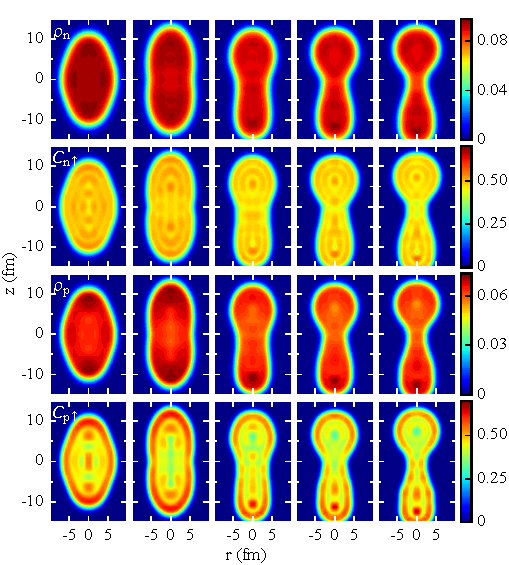
\includegraphics[width=0.5\linewidth]{TeX_files/methods_locali}
	\caption[Proton and neutron densities (in nucleons/fm$^3$) and spatial localizations for $^{240}$Pu at several configurations along the most-probable path to fission.]{Proton and neutron densities (in nucleons/fm$^3$) and spatial localizations for $^{240}$Pu at several configurations along the most-probable path to fission. Figure from~\cite{Zhang2016}.}
	\label{fig:methodslocali}
\end{figure}

As demonstrated in Figure~\ref{fig:methodslocali}, the NLF offers greater insight into the underlying shell structure of a system than the nucleon density. In particular, when applied to fission as in~\cite{Sadhukhan2017}, it enables one to see the formation of well-defined prefragments whose shell structure is responsible for the peak of the fragment distribution.


\section{Microscopic description of nuclear fission}\label{sect:fissionmethod}
With a nuclear many-body method now in hand, it can be used as a tool to describe fission. Recently in~\cite{Sadhukhan2016}, a nuclear DFT-based approach based on this assumption was used to compute fragment yields from a PES that was computed self-consistently, using the WKB approximation to describe tunneling and Langevin dynamics to describe post-tunneling dissipation. The half-life can be computed as in~\cite{Sadhukhan2013}. The entire procedure, illustrated schematically in Figure~\ref{fig:methodsoverview}, is described below.

\begin{figure}
	\centering
	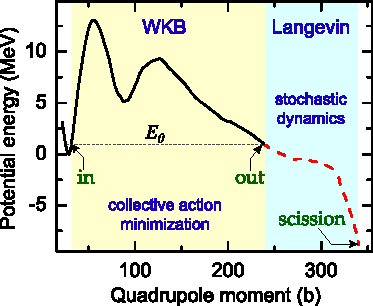
\includegraphics[width=0.5\linewidth]{TeX_files/methods_overview}
	\caption[Schematic overview of the Langevin framework for fission calculations used in this dissertation]{Schematic overview of the Langevin framework for fission calculations used in this dissertation. Figure from~\cite{Sadhukhan2016}.}
	\label{fig:methodsoverview}
\end{figure}

\subsection{Potential energy surfaces}
The primary degrees of freedom in the adiabatic approximation are nuclear collective shapes, and the basic ingredient to fission calculations is a PES. One could describe any nuclear configuration using a sufficiently-detailed PES; however, for practical computations one must use a truncated set of only a few collective coordinates. Thus, an important challenge for researchers is to select the most relevant collective coordinates, ideally while demonstrating that others can be safely neglected. Often, one will use the first few lowest-order moments, but there is some discussion within the community about whether these are the best for describing configurations on the way to fission, especially near scission (see, for instance,~\cite{younes2012}). Other collective coordinates which are sometimes used in the literature include $q_N$, which controls the size of the neck, and non-geometric variables which control pairing and pairing fluctuations such as the pairing gap $\Delta$ or $\left\langle \Delta \hat{N}^2 \right\rangle$, the mean value of particle number fluctuations.

Once the appropriate collective-coordinate constraints $\vec{q}\equiv(q_1, q_2, \dots)$ are chosen, the PES is computed on a mesh: one DFT calculation per grid point. The density at each point $\vec{q}$ is then used to compute the HFB energy $E'(\vec{q})$~\eqref{eq:routhian}.

\subsection{Collective inertia}
Just as important as potential energy to the fission dynamics is the collective inertia, which describes the tendency of the system to resist configuration changes (such as shape changes)~\cite{Hill1953}. The form of the collective inertia used here is the non-perturbative adiabatic time-dependent HFB (ATDHFB) inertia with cranking~\cite{Baran2011}, which takes the form
\begin{equation}\label{eq:mATDHFB-np}
\mathsf{M}_{\mu\nu} =  \frac{\hbar^2}{2}\frac{1}{(E_a+E_b)}\left(\frac{\partial\mathcal{R}^{21}_{(0),ab}}{\partial q_\mu}\frac{\partial\mathcal{R}^{12}_{(0),ba}}{\partial q_\nu}+\frac{\partial\mathcal{R}^{12}_{(0),ab}}{\partial q_\mu}\frac{\partial\mathcal{R}^{21}_{(0),ba}}{\partial q_\mu}\right),
\end{equation}

\noindent The subscripts and superscripts are explained in the full temperature-dependent derivation of the collective inertia found in Appendix~\ref{append:TD-ATDHFB}, but an important feature to note is that computing the inertia requires differentiating the density matrix with respect to a pair of collective coordinates. In expressions where the collective coordinates are shape degrees of freedom, the collective inertia acts as a masslike term to resist changes to the collective motion.

A perturbative expression for the ATDHFB inertia also exists, which allows one to estimate the inertia without taking derivatives of the density~\cite{Baran2011}. It is computationally much faster and easier to implement, but it loses many of the important features of the inertia compared to the non-perturbative case, as we shall see in Chapter~\ref{chap:294Og}. Nevertheless, it is commonly-used in calculations and later on we shall show how this choice affects fission yields compared to the non-perturbative inertia.

Another common expression for the collective inertia comes from the Generator Coordinate Method (GCM). The GCM inertia also exists in two varieties: perturbative and non-perturbative~\cite{giuliani2018b}. Like the ATDHFB inertia, the perturbative GCM inertia is smoothed-out compared to the non-perturbative inertia. Both the perturbative and non-perturbative GCM inertias are found to be smaller in magnitude than their ATDHFB counterparts.

\subsection{WKB approximation}\label{sect:wkb}
Spontaneous fission is an extreme case of quantum tunneling. If the wave function of the fissioning nucleus is assumed to be slowly varying inside the (large) potential barrier (which condition is satisfied under the adiabatic assumption), then the WKB approximation allows us to estimate the probability of tunneling through a classically-forbidden region in the PES.

Under the WKB approximation, the most-probable tunneling path $\left. L(s) \right|_{s_{\rm in}}^{s_{\rm out}}$ in the collective space is found via minimization of the collective action
\begin{equation}\label{eq:action} 
S(L) = \frac{1}{\hbar}\int_{s_{\rm in}}^{s_{\rm out}} \sqrt{2\mathcal{M}(s)\left(E'(s)-E_0\right)}ds,
\end{equation} 

\noindent where $s$ is the curvilinear coordinate along the path $L$, $\mathcal{M}(s)$ is the effective collective inertia given by~\cite{Sadhukhan2013}
\begin{equation}
\mathcal{M}(s) = \sum_{\mu\nu} \mathsf{M}_{\mu\nu} \frac{dq_\mu}{ds} \frac{dq_\nu}{ds}
\end{equation}

\noindent and $E'(s)$ is the potential energy along $L(s)$. $E_0$ stands for the collective ground-state energy. The calculation is repeated for different outer turning points, and each of these points is then assigned an exit probability $P(s_{\rm out})=[1+\exp{2S(L)}]^{-1}$~\cite{Baran1978}. 

The half-life corresponds to the pathway of minimum action, and the expression for the half-life is $T_{1/2} = \mathrm{ln}(2)/nP(s_\mathrm{min})$, where the parameter $n$ is the number of assaults on the fission barrier per unit time and which we set to the standard value $n=10^{20.38} s^{-1}$~\cite{Baran1978}. However, because of the exponential dependence of the half-life on the action, half-life calculations suffer from large uncertainties due to the uncertainties in theoretical ingredients.

\subsection{Langevin dynamics}

Although the link between collective and intrinsic degrees of freedom was assumed away in the adiabatic approximation, it is necessary to reintroduce some connection between the two, especially in the region between the outer turning points and scission where the adiabatic assumption is weakest. Through the semiclassical Langevin approach~\cite{Kubo1966}, we introduce a dissipation tensor $\eta$ that mimics energy exchange between intrinsic and collective modes. The dissipation tensor is related to a random force with strength $g$ via the fluctuation-dissipation theorem~\cite{Callen1951,Kubo1966}: $\sum_k g_{ik}g_{jk} = \eta_{ij}k_BT$. The fluctuation-dissipation theorem effectively couples collective and intrinsic degrees of freedom via the system temperature $T$, given by $k_BT = \sqrt{E^*/a}$ where $a=A/10$MeV$^{-1}$ parameterizes the level density and the excitation energy is given by $E^*(\vec{q}) = E'(s_{out}) - E'(\vec{q}) - \frac{1}{2}\sum\left(\mathcal{M}^{-1}\right)_{ij}p_i p_j$ (see~\cite{Abe1996,Frobrich1998,Sadhukhan2016} for details).

After emerging from the classically-forbidden region of the PES, fission trajectories proceed across the PES from the outer turning line, evolving according to the Langevin equations:
\begin{gather}\label{eq:langevin} 
	\frac{dp_i}{dt} =  
	-\frac{p_j p_k}{2} \frac{\partial}{\partial q_i}\left(\mathcal{M}^{-1}\right)_{jk} 
	- \frac{\partial E'}{\partial q_i}  - \eta_{ij}\left(\mathcal{M}^{-1}\right)_{jk} p_k + g_{ij}\Gamma_j(t) \,, \\ 
	\frac{dq_i}{dt} = 	\left(\mathcal{M}^{-1}\right)_{ij} p_j \,,  
\end{gather} 
\noindent where $p_i$ is the collective momentum conjugate to $q_i$, and $\Gamma_j(t)$ is a Gaussian-distributed, time-dependent stochastic variable. From here one can see that the dissipation term\\\noindent $- \eta_{ij}\left(\mathcal{M}^{-1}\right)_{jk} p_k$ represents a transfer of energy from the collective motion of the system to intrinsic single particle degrees of freedom, while the random fluctuation term $g_{ij}\Gamma_j(t)$ does the opposite.

Dissipation is treated in our work phenomenologically, since a self-consistent description of dissipation has not yet been fully developed~\cite{Bulgac2018a}.  In the meantime, we use the values of the dissipation tensor from~\cite{Sadhukhan2016}, which were fitted to reproduce the $^{240}$Pu spontaneous fission fragment yields.% However, work along this line has been started (maybe?) in refs 291-293 of~\cite{Schmidt2018} (see Section 4.1.1 for the context).

\subsection{Fragment identification via localization function}\label{sect:FragID}
The Langevin approach represents the best of what static approaches currently have to offer in terms of quantitative reproduction of the yields; however, it can be expensive and time-consuming to perform a full Langevin calculation with non-perturbative collective inertia in a multidimensional collective space. For applications where the level of quantitative accuracy is somewhat flexible (an example would be r-process network calculations, which are explained in Chapter~\ref{chap:rprocess}), one might ask whether it is necessary to do all these calculations if simple predictions are required (e.g., most-probable fission yields), or if there is some kind of physical insight that can be leveraged to reduce the workload.

By studying nucleon localization functions (Section~\ref{sect:locali}) for deformed configurations of fissioning nuclei, we observe that, in many cases, two distinct fragments start to form independently and then separate well before scission is reached (see Figure~\ref{fig:methodslocali}, taken from~\cite{Zhang2016}, as well as Sections~\ref{sect:178Ptfrags} and~\ref{sect:294Ogfrags}). Thus, a fissioning nucleus can be thought of as two well-formed prefragments connected by a neck. At scission, the two prefragments separate and the remaining neck nucleons are distributed to either of the two prefragments in some predictable way. Based on this, we developed a prescription for identifying prefragments and then estimating fragment yields at the outer turning line, using a statistical technique based on the grand canonical ensemble. This prescription is described in Appendix~\ref{append:Fragments}. % Intro to nuclear DFT
\chapter{Numerical Implementation}\label{chap:Numerical}

Since this modern era of fission theory takes advantage of high-performance computers, it is worth taking some time to discuss some of the issues which came up during the course of this research, and how modern computing tools were used to solve the problem.

\section{Calculating the PES}
By far, the most time-intensive part of a microscopic fission calculation is the calculation of the PES. For this we use a pair of DFT solvers, HFODD \cite{Schunck2017} and HFBTHO \cite{Perez2017}. These programs solve the HFB equations in a basis of deformed harmonic oscillators. The solver HFBTHO is limited to shapes with axial symmetry, while HFODD allows for the breaking of any symmetry needed. Broken symmetries mean that each matrix element must be computed independently, while good symmetries mean However, since the major bottleneck of each of these programs involves constructing matrices representing Skyrme densities and currents and then diagonalizing the matrix representing the HFB Hamiltonian, this flexibility drastically increases the time-to-solution.

On the positive side, the problem of calculating a PES is embarrassingly-parallel. So while an individual point in the PES may be difficult to compute, many points can be computed simultaneously. This does have its limitations; highly-deformed configurations may be very unstable because of reasons. One fix may sometimes be to use a nearby point which converged successfully as a seed function

The procedure is performed iteratively: First, an ansatz is given for the density (either by the user or by some simple means, such as a quick Woods-Saxon calculation). Then the energy density matrix is constructed, after which it is diagonalized and a new density matrix is calculated. The procedure then repeats for a fixed number of iterations, or until a predetermined convergence criterion is satisfied In HFODD, for instance, the default convergence criterion is for the difference between the total energy summed over all single-particle states and the total energy calculated by \verb|???| to be less than some user-defined value.

Certain parts of the procedure can be parallelized using shared-memory parallelism, such as QMULCM, which does what again? It readjusts the Lagrange parameters of the constraints based on the perturbative approximation fot he QRPA matrix.

\subsection{PES Tools}
Apart from the issue of walltime, generating a PES creates a lot of output files, which quickly becomes unwieldy. To help manage all this data, a Python module called PES Tools was created for manipulating, extracting, interpolating, and plotting PES data \cite{PES_tools}. Aside from solver-dependent parser scripts, which collect data from the output of a DFT run and store it in the XML file format, PES Tools is not dependent on a particular DFT solver.

In particular, a submodule was created to interface between PES Tools and Fission Tools \cite{fission_tools}, a set of codes which have relevance to fission calculations. Many of these codes are described in the following sections.

\section{Calculating the collective inertia}\label{sect:M_numerical}
The partial derivatives from equation \ref{eq:mATDHFB-np} are computed using the Lagrange three-point formula:

\begin{equation}\label{eq:finite-diffs}
\left(\frac{\partial \mathcal{R}}{\partial q}\right)_{q=q_0} \approx 
    \frac{-\delta q'}{\delta q \left(\delta q + \delta q'\right)}\mathcal{R}(q_0-\delta q) + 
    \frac{\delta q - \delta q'}{\delta q \delta q'}\mathcal{R}(q_0) + 
    \frac{\delta q}{\delta q' \left(\delta q + \delta q'\right)}\mathcal{R}(q_0+\delta q')
\end{equation}

The accuracy and precision of the collective inertia $\mathcal{M}$ are therefore functions of the spacings $\delta q$ and $\delta q'$, and of $\mathcal{R}$. An accurate value of the collective inertia is especially important for computing half-lives, where there is an exponential dependence on $\mathcal{M}$.

\begin{figure}
	\centering
	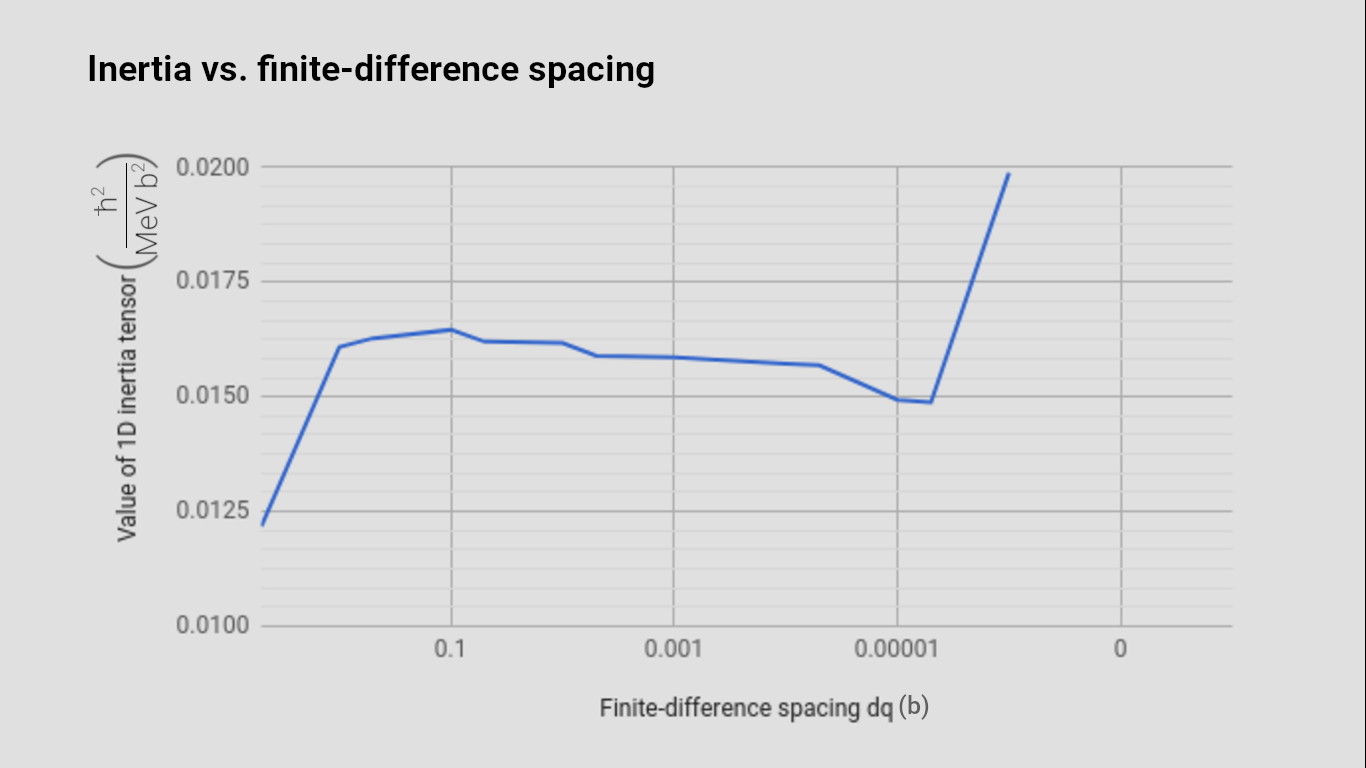
\includegraphics[width=0.7\linewidth]{TeX_files/Num-dq_spacing}
	\caption[Collective inertia as a function of finite-difference spacing]{$\mathcal{M}_{22}$ calculated for ??? configuration of $^{240}$Pu as a function of finite-difference spacing.}
	\label{fig:num-dqspacing}
\end{figure}

Figure \ref{fig:num-dqspacing} shows the effect of different values of $\delta q = \delta q'$ on the collective inertia for a particular configuration of $^{240}$Pu.

\begin{figure}
	\centering
	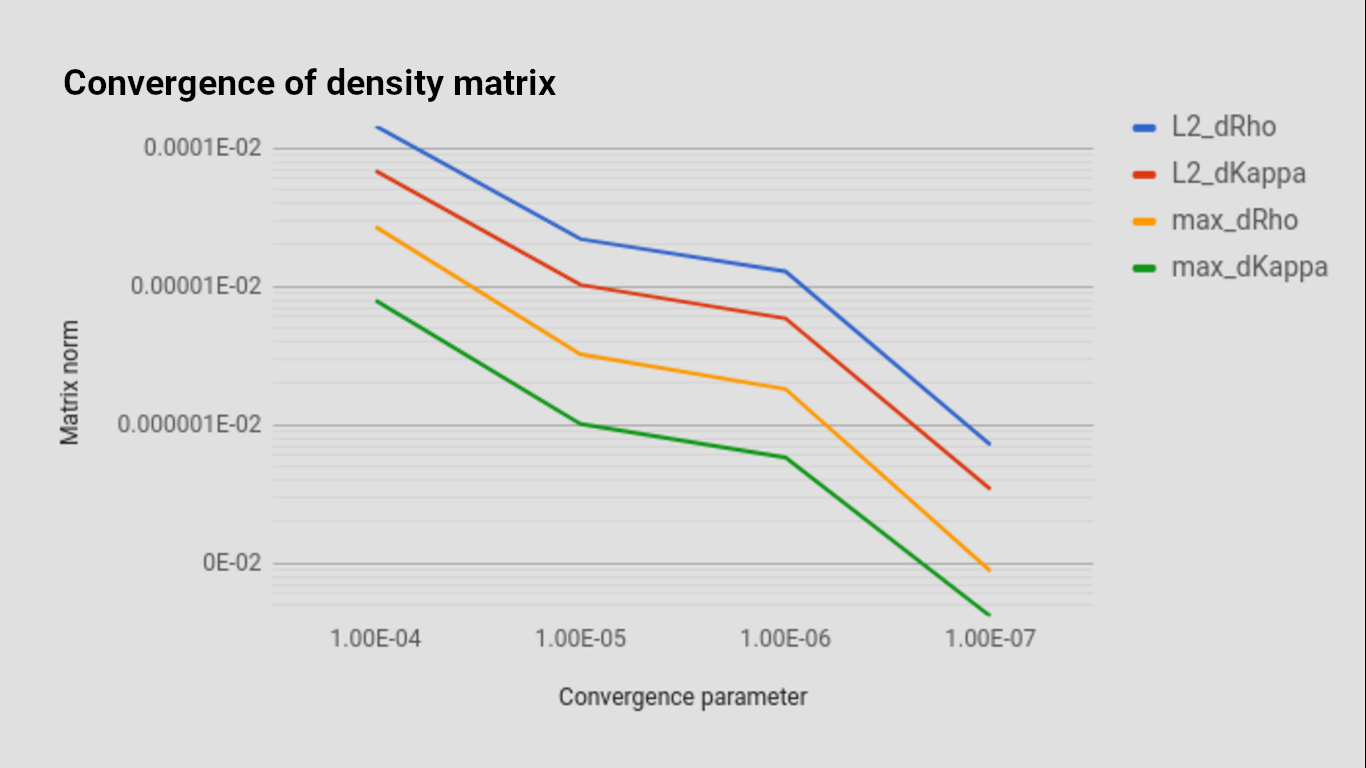
\includegraphics[width=0.7\linewidth]{TeX_files/Num-rho_conv}
	\caption[Norm of the difference matrix between subsequent iterations of the density]{Norm of the difference matrix between subsequent iterations of the density.}
	\label{fig:num-rhoconv}
\end{figure}

Figure \ref{fig:num-dqspacing} shows the norm of the matrix which corresponds to the difference between the density matrix at the last iteration and the second-to-last iteration. Predictably, the norm decreases as the convergence parameter becomes tighter. This gives a sense of the uncertainty associated with the density, which in turn should be propagated through equations \ref{eq:finite-diffs} and \ref{eq:mATDHFB-np}.

There are additional complications which arise in the finite-temperature formalism. These are discussed in Appendix \ref{append:TD-ATDHFB}.

\section{Minimum action path}
For the tunneling described in Section \ref{sect:wkb}, the dynamic programming method \cite{Baran1981} was used to minimize the action. The dynamic programming scheme proceeds inductively: Once the minimum action is known for all grid points up to a certain value of $Q_{20}$, say $q_{20}^n$, then the minimum action at each grid point in the layer with $Q_{20}=q_{20}^{n+1}$ is obtained by computing the action between each grid point in layer $n$ and each grid point in layer $n+1$, and then finding the path which minimizes the total action at each grid point in layer $n+1$:

\begin{equation}
\left.S_{min}(\vec{Q})\right|_{Q_{20}=q_{20}^{n+1}} = \mathrm{argmin}_{\vec{Q'}}\left.\left(S_{min}(\vec{Q'}) + \Delta S_{min}(\vec{Q},\vec{Q'})\right)\right|_{Q'_{20}=q_{20}^{n}, Q_{20}=q_{20}^{n+1}}.
\end{equation}

The inductive step which connects layers $n$ and $n+1$ involves several small, independent calculations which lend themselves well to shared-memory parallelism. This was implemented in the code using OpenMP, resulting in a walltime reduction from order $\mathcal{O}(n^D)$ to $\mathcal{O}(n^D/m)$, where $m$ is the number of processors (with the usual caveats that parallelization requires some additional overhead time, and that the actual speedup might be somewhat less when the number of processors $m$ reaches the same order as the number of points per layer $n^{D-1}$). In a 2D calculation, where the runtime is on the order of seconds, the difference is inconsequential. However, this speedup was essential for the analysis of a 4D PES, as described in Chapter \ref{chap:294Og}.


\section{Langevin}
Once the action and relative probability are known for a set of points along the outer turning line, Langevin trajectories are computed originating from each outer turning point. These are straightforwardly evaluated at discrete time steps over a discretized PES mesh.

Because of the random force term in equation \ref{eq:langevin}, a large number of trajectories per outer turning point must be computed to reduce statistical uncertainty. Fortunately, each trajectory is completely independent of every other trajectory, lending the code readily to shared-memory parallelism. However, for the Fission Tools Langevin code I chose to use distributed-memory parallelism instead of shared-memory parallelism in order to simplify access to shared resources, such as variables and output files. % Two fission modes in 178Pt
\chapter{Two fission modes in $^{178}$Pt}\label{chap:178Pt}

\section{Asymmetric fission in the region of $^{180}$Hg}
As mentioned in the introduction, fission has been studied most carefully in the region of the actinides (Z=90 to Z=103), as many naturally-occurring isotopes in this region are fissile. Within this region, there is a characteristic tendency for fission fragment yields to be asymmetric (that is, one light fragment and one heavy fragment), with the heavy peak centered around $A\approx140$. This has been understood as a manifestation of nuclear shell structure in the prefragments: doubly-magic $^{132}$Sn drives the nucleus towards scission, and once the neck nucleons are divided up between the two fragments, the heavy fragment distribution peaks near A=140. As one moves to the lower-Z actinides, however, this tendency becomes less and less pronounced as yields tend to become more symmetric. Until recently, it was generally believed that below thorium, yields would continue to be symmetric. For sub-thorium isotopes, there was no doubly-magic nucleus candidate that could drive the system toward asymmetry as there is with actinides.

However, it was reported in a 2010 study \cite{Andreyev2010} that neutron-deficient $^{180}$Tl undergoes beta-delayed fission, leading to intermediate state {\Hg} which then decays into two fragments of unequal mass. This finding triggered a flurry of theoretical papers hoping to describe this new and unexpected phenomenon (for instance, see \cite{Warda2012,Moller2012,Mcdonnell2014,Ichikawa2019}). A follow-up study using $^{178}$Tl \cite{Liberati2013} further established this as a region of asymmetric fission, and not just a one-time occurrence. Since then, other nuclei in the region have been studied using a variety of reactions and techniques, and the finding is the same. 

%Nuclei in this region have a number of unique features which make them interesting for study, even aside from the unexpected fragment asymmetry. Predicted fission barrier heights in this region are relatively-low (of the order of ~12 MeV), making them suitable for study using low-energy techniques such as $\beta$-delayed fission (maybe \cite{Andreyev2013} and the work at ISOLDE at CERN?) or Coulex-induced fission (maybe \cite{Martin2015} and the SOFIA (Studies On FIssion with Aladin) experiment/project/campaign). On the other hand, it has been found that compound nuclei formed in this region from particle-induced reactions tend to have high excitation energies, even for beam energies near the Coulomb barrier. This combination makes the region particularly well-suited for studies involving a variety of excitation energies.

Later experiments have shown that, unlike the case of actinides where shell structure and fragment asymmetry are ``washed out'' at high excitation energies, mass asymmetric fragment distributions are a persistent feature of this mass region for various excitation energies (see \cite{Andreyev2018} and references therein). An overview of nuclei in the region of {\Hg} which have been experimentally studied (as of 2016), including the experimental technique used, is shown in Figure \ref{fig:178ptregion}.

\begin{figure}
	\centering
	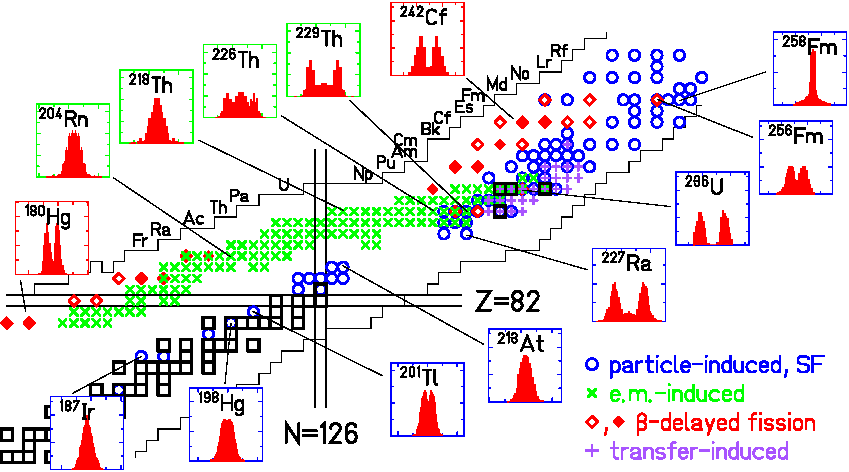
\includegraphics[width=0.9\linewidth]{./TeX_files/178Pt_region}
	\caption[Survey of fragment yields near $^{180}$Hg]{Fragment yields for several nuclei ranging from actinides, where primary fission yields tend to be asymmetric, down to near-thorium, where yields become more symmetric, and finally to the region near neutron deficient {\Hg}, where asymmetry returns. Figure from \cite{Andreyev2018}.}
	\label{fig:178ptregion}
\end{figure}



\section{Multimode fission of $^{178}$Pt}

One particular follow-up experiment was performed to investigate the spontaneous fission of {\Pt} \cite{Tsekhanovich2019}, which differs from {\Hg} by 2 protons. This system was studied at various excitation energies and found to fission consistently in a bimodal pattern, as shown in Figure \ref{fig:178ptexptdata}. Of the sample measured, roughly 1/3 of cases were found to fission symmetrically, while the other 2/3 fissioned asymmetrically with a light-to-heavy mass ratio of approximately 79/99. Furthermore, it was observed that mass-asymmetric fragments tended to have higher kinetic energies than symmetric fragments.

\begin{figure}
	\centering
	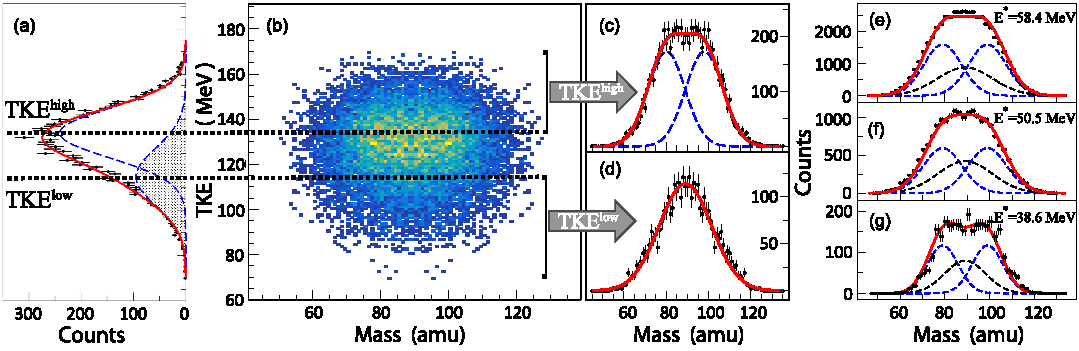
\includegraphics[width=0.95\linewidth]{TeX_files/178Pt_expt_data}
	\caption[$^{178}$Pt experimental data]{After projecting the fission fragment mass vs total kinetic energy (TKE) correlation (a) onto the TKE axis, the TKE distribution is deconvoluted into high- and low-energy components, centered around the values TKE$^\mathrm{high}$ and TKE$^\mathrm{low}$ (b). The corresponding mass distributions are fitted to a double (c) and single (d) Gaussian, respectively. This procedure is repeated for three different compound nucleus excitation energies E* (e-g). Figure from \cite{Tsekhanovich2019}}
	\label{fig:178ptexptdata}
\end{figure}

To better interpret the results of this experiment, DFT calculations were performed using the functionals {\hfb} \cite{Schunck2015} and D1S \cite{Berger1989}. These calculations involved computing a PES using the collective coordinates $Q_{20}$ and $Q_{30}$. The {\hfb} PES is shown in Figure \ref{fig:178ptunedf1pes}, while the D1S PES is in Figure \ref{fig:178ptd1spes}. A calculation with full Langevin dynamics was not performed; however, the static (minimum-energy) pathways shown in the figures correspond to a fragment split $A_L/A_H \approx 80/98$.

\begin{figure}
	\centering
	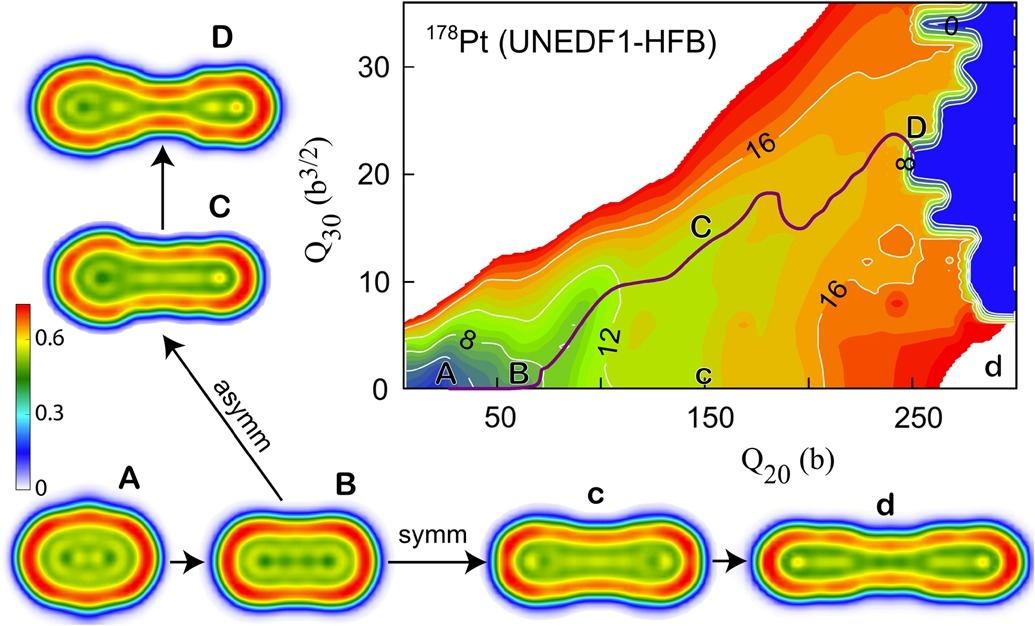
\includegraphics[width=0.7\linewidth]{TeX_files/178Pt_unedf1_pes.jpg}
	\caption[UNEDF1-HFB potential energy surface for $^{178}$Pt]{UNEDF1-HFB potential energy surface for $^{178}$Pt. Note the two different trajectories ABCD and ABcd and their corresponding localizations.}
	\label{fig:178ptunedf1pes}
\end{figure}

Also shown in Figure \ref{fig:178ptunedf1pes} are nucleon localization functions (recall Section \ref{sect:locali}) corresponding to various marked configurations in the PES. Along the symmetric path (ABcd in the figure), the fragments appear highly-elongated, even shortly before scission. Since elongation tends to minimize the Coulomb repulsion between fragments, then this configuration might be expected to lead to fragments with relatively low kinetic energies. On the other hand, compact fragments such as those in ABCD will tend to have a larger Coulomb repulsion. Fragments will be propelled away from one another with greater force, resulting in fragments with a higher kinetic energy, which is in qualitative agreement with experiment.

Comparing the {\hfb} PES in Figure \ref{fig:178ptunedf1pes} to the D1S PES in Figure \ref{fig:178ptd1spes}a, one may note that, despite the inherent differences between the functionals, the overall topology of the PES is similar in both cases. In fact, the topology in both cases is quite flat, which suggests (in agreement with the observed data) the possibility of a competition between symmetric and asymmetric fission modes. Additionally, as shown in Figure \ref{fig:178ptd1spes}b, there appears an additional channel corresponding to compact symmetric fragments. This channel is higher in energy than the elongated symmetric pathway and is blocked by a $\sim4$ MeV saddle point, but it is conceivable that this channel might be more easily accessed by other isotopes in this region.

\begin{figure}
	\centering
	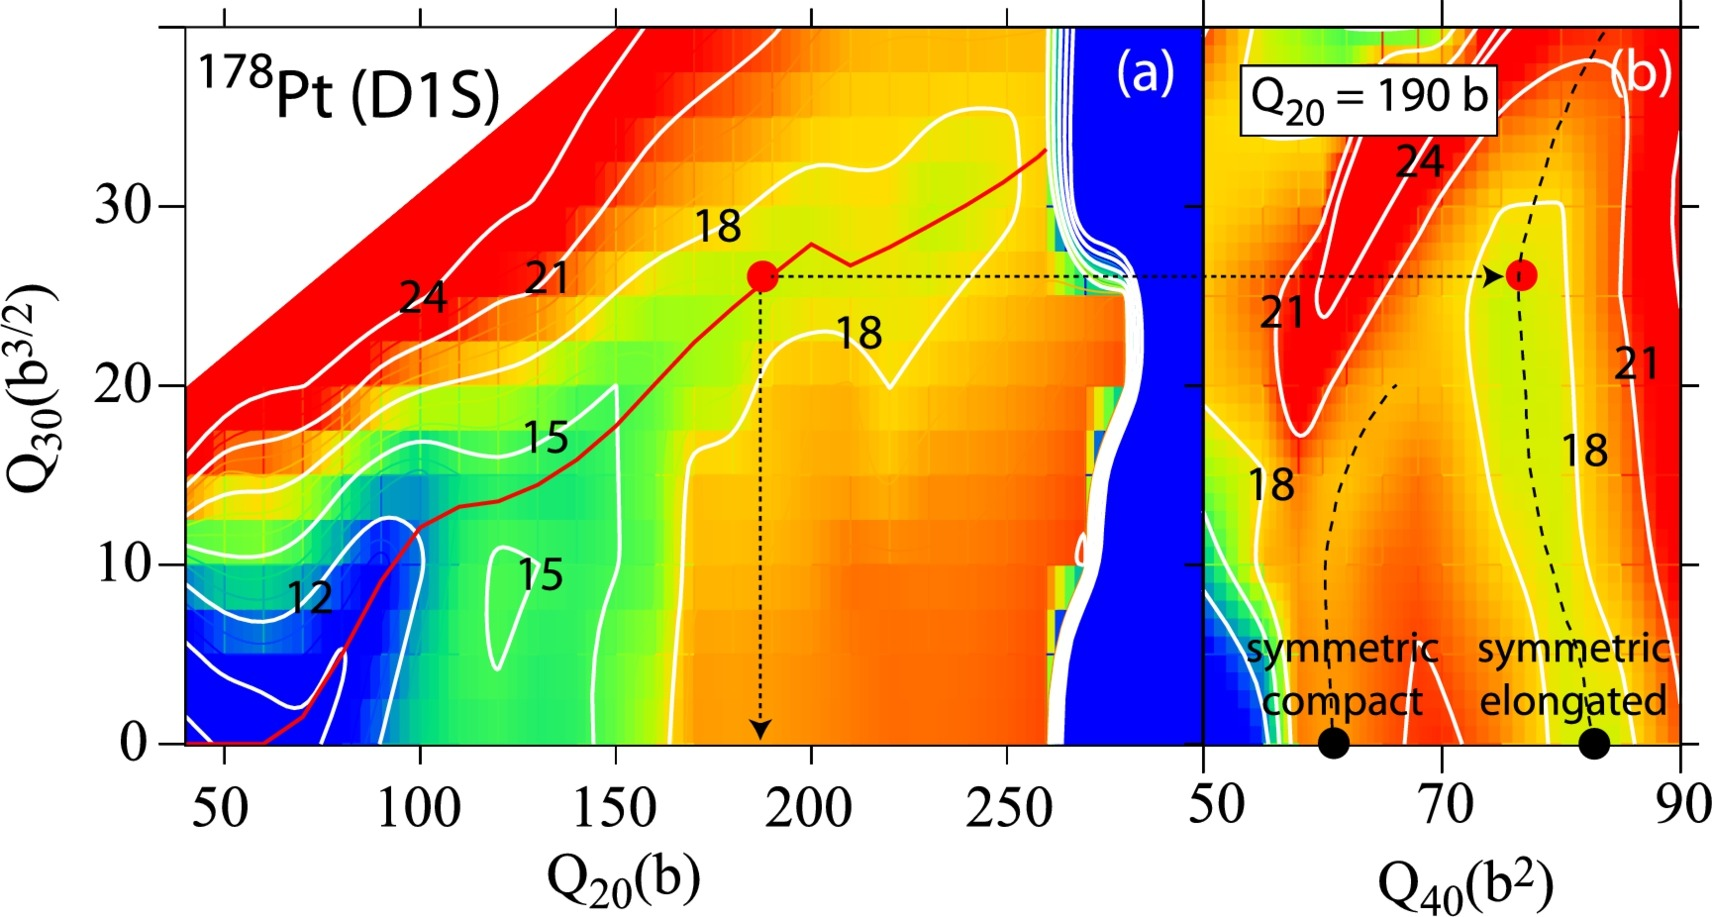
\includegraphics[width=0.7\linewidth]{TeX_files/178Pt_D1S_pes.jpg}
	\caption[D1S potential energy surface for $^{178}$Pt]{D1S potential energy surface for $^{178}$Pt. Note also the additional information about the hexadecapole moment.}
	\label{fig:178ptd1spes}
\end{figure}



\section{The physical origin of fragment asymmetry in the region of $^{180}$Hg}

Why is there a region of symmetric fission below thorium?

(These are notes from the 178Pt paper draft. Not mine, of course, but they have some good points to address): ``Namely, the PES are predicetd to be flat and much less structureless, and defined predominantly by the large liquid drop/macroscopic contribution, rather than by relatively small microscopic effects. Due to this, FFMDs exhibit fairly low dependence..  [refer to 180Hg PLB, as one example].

``(this was an answer by Witek, when somebody asked a question to my talk at Tsukuba - why the lead region is less sensitive to temperature.. the answer was - there is no 'barrier' in a sence, it's just flat/thick macroscopic surface, hardly influenced by shell effects.. so, even if one heats it up, tiny shell effects will be gone, but the main underlying macroscopic part will remain).''

Peter Moller argues in the concluding discussion of (https://link.aps.org/doi/10.1103/PhysRevC.85.024306 \cite{Moller2012}) that we can't really use the fragment/prefragment shell structure arguments in this region, and thus that we have yet to identify all the essential physics which determines fragments. He says the yields are given (at least in this case) by subtle interplays in local regions of the potential energy surface. He also has another paper \cite{Ichikawa2019}.

Witek, Michal Warda, and Staszczak argue in Section IV. \textit{Prescission Configurations} of \cite{Warda2012a} that 180Hg deforms as a molecular system consisting of 90Zr and 72Ge, with the remaining neck nucleons being distributed at scission to give the fragments they found in the experiment. Similarly, they make the same claim for 198Hg, except using 98Zr and 80Ge. The first one kind of makes sense to me since 90Zr is semi-magic, but 98Zr is not and neither is 80Ge. I wonder what might have happened had they tried to match up the densities of a different set of nearby nuclei (they used these because they had the same N/Z ratio as the fissioning parent nucleus). Then in the conclusions: ``We conclude that the mass distribution of fission fragments in both nuclei is governed by shell structure of prescission configurations associated with molecular structures.''

Scamps and Simenel claim at the end of \cite{Scamps2018a} that perhaps the asymmetry can be explained by shell closures in octupole-deformed fragments, rather than spherical magic numbers.

In the introduction to \cite{Mcdonnell2014} it is stated as though conclusively that ``the main factor determining the mass split in fission are shell effects at pre-scission configurations, i.e., between saddle and scission'' (see also some additional references therein). I think the thing that is most selling it to me so far, though, is Fig. 3 from this paper, wherein they show the shell correction energy for each of the nuclei considered. Even though the PES itself is mostly flat in each of these cases, the magnitude of the shell correction is different whether you are looking at symmetric or asymmetric trajectories, and the one with the larger magnitude shell correction happens to be the one that wins out in the final fragment distribution. I'd also be curious to see what the collective inertia looks like, but this seems to at least give something. It's not like this shell correction gets added on top of the PES - the PES is still relatively-flat - but it at least gives an explanation for why our traditional physical intuition is not totally failing us here.

Interesting future work in this region might include calculations with full dynamics (including from nuclei with excitation energy), as suggested in the conclusions of \cite{Mcdonnell2014}






 % Cluster decay in 294Og
\chapter{Cluster decay in $^{294}$Og}\label{chap:294Og}

\section{Cluster emission in superheavy elements}

The region of superheavy elements, defined as the set of nuclides with $Z>104$, is an interesting one for the study of spontaneous fission because the liquid drop model predicts that all isotopes with $Z>104$ are unstable with respect to spontaneous fission. These nuclei receive additional stability due to shell effects, but they nevertheless remain short-lived and many of them will decay by spontaneous fission regardless.

Experimentally, spontaneous fission has been observed from several superheavy isotopes (those marked in green in the right panel of Figure~\ref{fig:karpovshedecay}). Other observed superheavy elements undergo a chain of several alpha decays followed by spontaneous fission. Furthermore, a variety of models predict regions where spontaneous fission dominates in the superheavy regime. One example is shown in the left panel of Figure~\ref{fig:karpovshedecay}, in which branching ratios were estimated by computing and comparing different decay lifetimes obtained from empirical formulas. Figure~\ref{fig:warda2012she} is similar, except that the spontaneous fission lifetimes were computed microscopically, as were the $Q_\alpha$ values used to estimate alpha decay lifetimes.


\begin{figure}
	\centering
	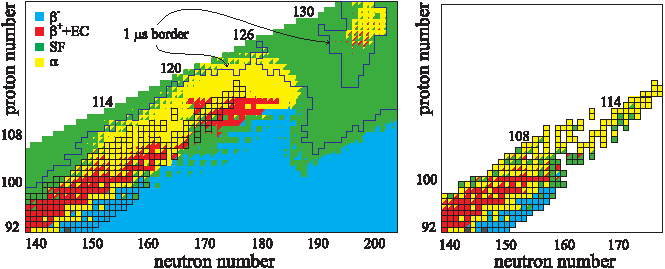
\includegraphics[width=0.9\linewidth]{TeX_files/294Og_Karpov_SHEdecay}
	\caption[Calculated (left) and experimental (right) decay modes for heavy and superheavy elements. The theoretical estimates are based on an analysis of lifetimes calculated via empirical formulae. The boxed isotopes in the left panel are those which have been measured experimentally. Isotopes falling inside the 1$\mu$s contour are predicted to live longer than 1$\mu$s. Figure adapted from~\cite{Karpova}.]{Calculated (left) and experimental (right) decay modes for heavy and superheavy elements. The theoretical estimates are based on an analysis of lifetimes calculated via empirical formulae. The boxed isotopes in the left panel are those which have been measured experimentally. Isotopes falling inside the 1$\mu$s contour are predicted to live longer than 1$\mu$s. Figure adapted from~\cite{Karpova}.}
	\label{fig:karpovshedecay}
\end{figure}


\begin{figure}
	\centering
	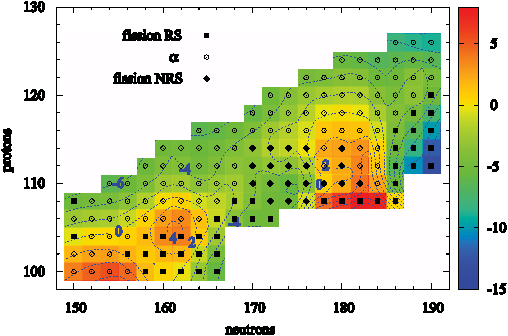
\includegraphics[width=0.7\linewidth]{TeX_files/294Og_Warda2012_SHE}
	\caption[Dominant decay modes for superheavy elements are indicated based on predictions obtained in a nuclear DFT-based framework.]{Dominant decay modes for superheavy elements are indicated based on predictions obtained in a nuclear DFT-based framework are indicated. The label ``RS'' stands for ``reflection symmetric'', meaning the least-action wavefunction at the saddle is reflection symmetric, and ``NRS'' stands for ``non-reflection symmetric.'' The colorbar indicates the predicted half-life on a logarithmic scale. Figure from~\cite{Warda2012}.}
	\label{fig:warda2012she}
\end{figure}

This still leaves open the question of fission fragments of superheavy elements, however. Several authors have predicted, using models both phenomenological~\cite{Poenaru2011, Poenaru2012, Poenaru2013, Poenaru2015, Poenaru2018,Santhosh2018, Zhang2018} and microscopic~\cite{Warda2018}, that some superheavy elements will undergo a highly-asymmetric form of fission in which the parent nucleus decays into two fragments, with the heavy fragment near the doubly-magic nucleus {\Pb}. This particular decay mode is significant enough to have earned its own name in the literature, where it is known variously as cluster emission, cluster radioactivity, or lead radioactivity~\cite{Sandulescu1980,Poenaru1986,Royer1998,Poenaru2010,Warda2011}. The phenomenon of cluster emission was first observed in 1984 in the decay $^{223}$Ra$\rightarrow$$^{209}$Pb + $^{14}$C~\cite{Rose1984} and has since been observed in several actinides. In all cases seen so far, it is a rare event with a small branching ratio~\cite{Poenaru2010}.

The mechanism of cluster emission is based on the stability of the doubly-magic nucleus {\Pb}. {\Og} is a particularly excellent candidate for cluster emission because the cluster it is predicted to emit, {\Kr}, receives additional stability due to its having a magic number of neutrons.  Semiempirical arguments based on the nuclear symmetry energy lend additional support to this candidate, since {\Og} and {\Pb} have a similar $N/Z$ ratio~\cite{Warda2018}.

We took this prediction one step further by calculating the full spontaneous fission fragment distribution of {\Og} using a microscopic approach. As will be shown, the distribution is sharply-peaked around {\Pb}, and this will be shown to be quite robust with respect to various inputs. A visualization of the process using the nucleon localization function shows strong evidence of a {\Pb} prefragment being formed early in the post-saddle stage of the evolution.

\section{Predicted spontaneous fission yields of $^{294}$Og}

Potential energy surfaces were computed for each of three EDFs: \hfb~\cite{Schunck2015}, a Skyrme functional which was optimized to data for spherical and deformed nuclei, including fission isomers; SkM*~\cite{Bartel1982}, another Skyrme functional designed for fission barriers and surface energy; and D1S~\cite{Berger1989}, a parameterization of the finite-range Gogny interaction fitted on fission barriers of actinides. A comparison of the different PESs as a function of multipole moments $Q_{20}$ and $Q_{30}$ is shown in Figure~\ref{fig:294ogthreepes}. Despite the quantitative differences between the functionals, one can see that the surfaces strongly resemble one another. Some common features we highlight are: a symmetric saddle point occurring around $Q_{20}\approx 40$\,b; a second barrier beginning around $Q_{20}\approx100-120$\,b along the symmetric fission path; the presence of local minima at large deformations (marked by stars in the figure); a deep valley that leads to an highly-asymmetric split; and a secondary, less-asymmetric fission valley that emerges at large elongations.


\begin{figure}
	\centering
	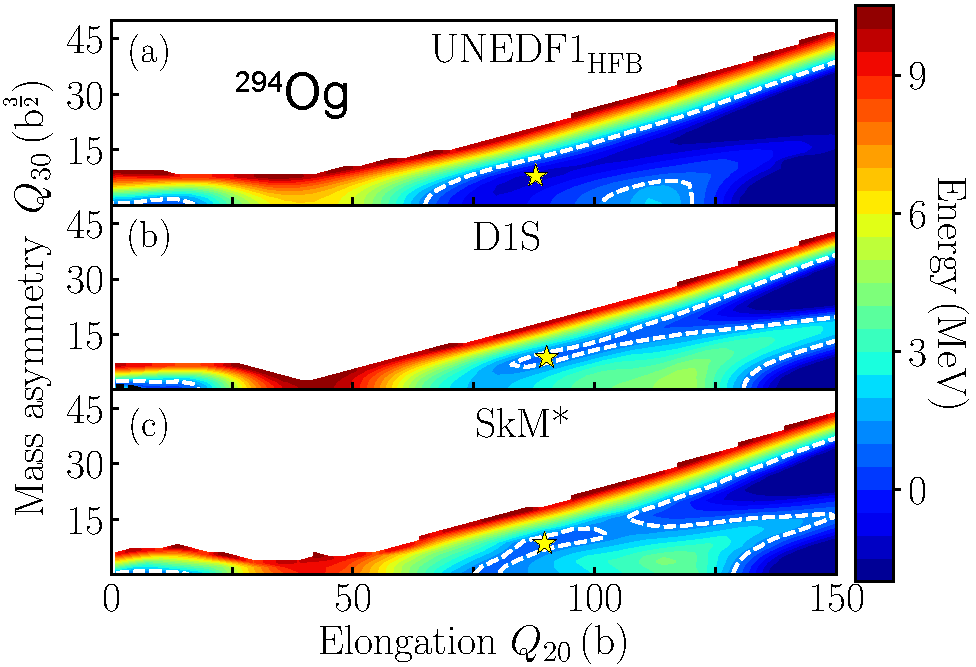
\includegraphics[width=0.7\linewidth]{TeX_files/294Og_three_PES}
	\caption[PES comparison for $^{294}$Og using EDFs {\hfb}, D1S, and SkM*.]{Comparison of the PESs for \Og{} in the $(Q_{20},Q_{30})$ collective plane obtained in \hfb{} (a), D1S (b), and SkM* (c) EDFs. The ground-state energy $E_{gs}$ is normalized to zero. The dotted line in each figure corresponds to $E_0-E_{gs}=1$\,MeV, which was used to determine the inner and outer turning points. The local energy minima at large deformations are marked by stars.}
	\label{fig:294ogthreepes}
\end{figure}

%% This passage is lifted straight from the paper, FYI
But there are differences as well, such as the height of the first saddle point, the depth of the highly-asymmetric fission valley, and the height of the ridge separating the two fission valleys. As a result, the outer turning points are pushed to larger elongations in D1S and SkM* as compared to \hfb{}. These differences in the PES topography strongly affect the predicted spontaneous fission half-lives $\tau_\mathrm{SF}$, which in the case of \hfb{}, SkM* and D1S are $9.1\times10^{-9}\,$s, $4.0\times10^{-5}\,$s and $3.2\times10^{-2}\,$s, respectively (see also~\cite{Staszczak2013,Baran2015} for a detailed discussion of half-lives). These large variations of $\tau_\mathrm{SF}$ reflect the well-known exponential sensitivity of spontaneous fission half-lives to changes in the quantities entering the collective action~\eqref{eq:action}. The $\tau_\mathrm{SF}$ predictions of \hfb{} and, to a lesser degree,  SkM* are incompatible with experiment, as $^{294}$Og  is known to  decay by $\alpha$-decay with a half-life of 0.58\,ms~\cite{Brewer2018}. The D1S result should not be taken too seriously, either, since they were performed in a smaller collective space leading to overestimation of the half-lives~\cite{Giuliani2014,Sadhukhan2014}.

It is to be noted that while half-lives are very sensitive to details of the calculations, the models used here are very consistent with each other and with experiment when it comes to global observables, such as alpha-decay energies, deformations, and radii~\cite{Heenen2015,Giuliani2019}. It will be demonstrated below that spontaneous-fission mass and charge yields are also robustly predicted (though experimental confirmation has not yet occurred). This robustness will be shown by varying the EDF, the collective space, the collective inertia, and the strength of the Langevin dissipation tensor (recall Section~\ref{sect:fissionmethod}).
%% End of lifted passage

The EDF and the collective space were varied together; a different collective space was used for each EDF in the tunneling portion of the PES. The {\hfb} calculation was carried out in a four-dimensional collective space consisting of the collective coordinates $(Q_{20}, Q_{30}, Q_{22}, \lambda_2)$. By examining this PES, we were able to reduce the dimensionality of the PES for the other two functionals. The SkM* calculation was performed in a piecewise-continuous space. Between the ground state and the isomer state, $Q_{30}$ does not play a significant role and so the system was described using  $(Q_{20}, Q_{22}, \lambda_2)$. Likewise, $Q_{22} \approx 0$ once the isomer state is reached and reflection symmetry is broken ($Q_{30} \neq 0$), suggesting use of the coordinates  $(Q_{20}, Q_{30}, \lambda_2)$. Finally, for the functional D1S we decided to see how our yields would be affected if we did not consider dynamical pairing fluctuations or axial symmetry breaking at all, which results in a drastic reduction to computation time. Those calculations were performed in the collective space $(Q_{20}, Q_{30})$.

In the region of Langevin dynamics, we found again that $Q_{22} \approx 0$. Consequently, this region was limited to two dimensions $(Q_{20}, Q_{30})$ in all cases.

\begin{figure}
	\centering
	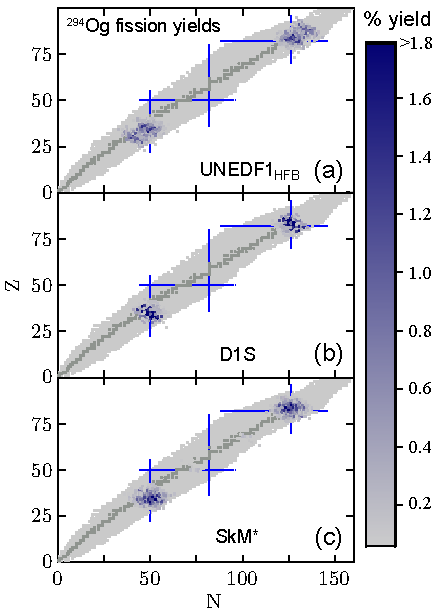
\includegraphics[width=0.9\linewidth]{TeX_files/294Og_3yields}
	\caption[N-Z fission fragment yields from $^{294}$Og]{Fission fragment distributions for \Og{} obtained in \hfb{} (a), D1S (b), and SkM* (c) EDFs using the non-perturbative cranking ATDHFB inertia and  the baseline  dissipation tensor $\mathbf{\eta}_0 = (\eta_{11},\eta_{22},\eta_{12}) = (50\hbar,40\hbar,5\hbar)$. Known isotopes are marked in gray~\cite{NuDat}. Magic numbers 50, 82, and 126 are indicated by dotted lines.}
	\label{fig:294og3yields}
\end{figure}

The resulting yields are shown in Figure~\ref{fig:294og3yields} as a function of $Z$ and $N$. As expected, the yields are peaked in the region of {\Pb} with a sharp fall-off. Likewise, the projected distributions onto the mass and charge axes show a clear preference for cluster emission, regardless of functional, as seen in the top panels of Figure~\ref{fig:294ogcompareall}.

\begin{figure}
	\centering
	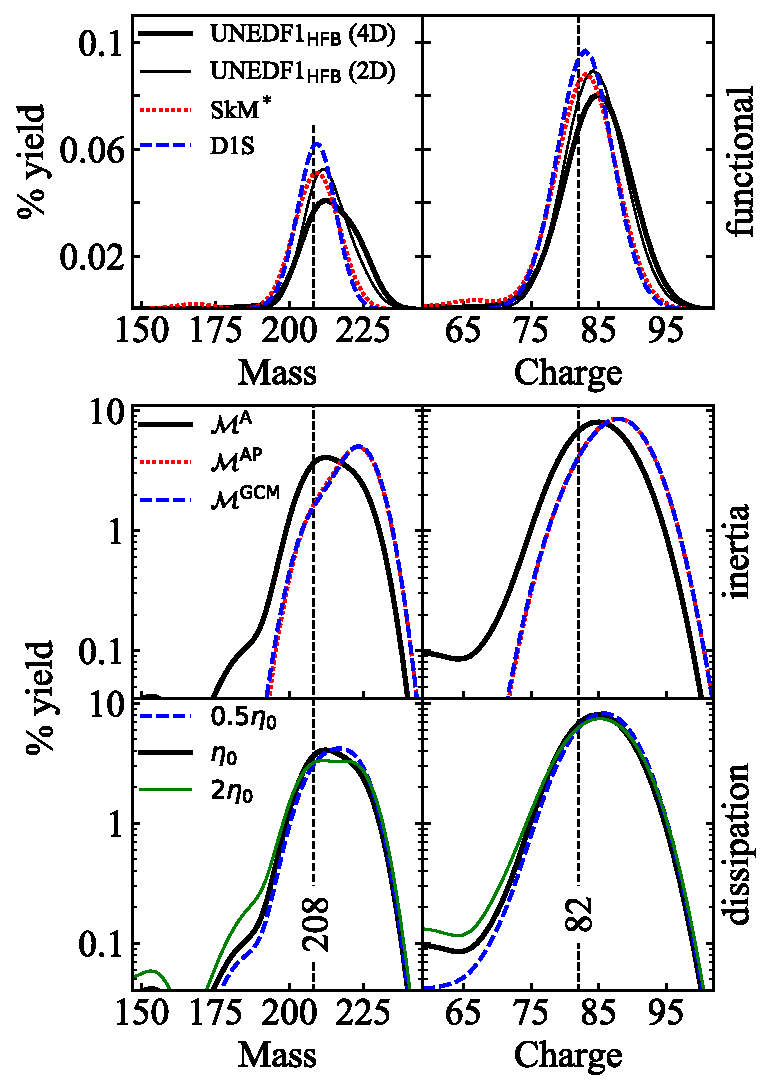
\includegraphics[width=0.7\linewidth]{TeX_files/294Og_compare_all}
	\caption[$^{294}$Og heavy fragment masses and charges.]{Upper panel: Predicted heavy fragment mass (left) and charge (right) yields of \Og{} using different functionals (top, linear scale). Lower panels: collective inertias (middle, logarithmic scale) and dissipation tensor strengths (bottom, logarithmic scale). The baseline calculation was performed using the \hfb{} functional in a 4D space with non-perturbative cranking ATDHFB inertia and dissipation tensor strength $\mathbf{\eta}_0$.}
	\label{fig:294ogcompareall}
\end{figure}

As discussed in Chapter~\ref{chap:Model}, the collective inertia can also have a large impact on the fission dynamics. Using the {\hfb} functional, we compared our result with the non-perturbative cranking ATDHFB inertia, {\MATDHF}, to two other expressions for the inertia which are computationally less expensive to compute and therefore commonly-used in large-scale calculations: the perturbative ATDHFB inertia {\MATDHFp} (which appears smoothed-out compared to {\MATDHF}~\cite{giuliani2018b}), and the perturbative GCM inertia {\MGCMp} (which is smooth and also lower in magnitude than {\MATDHF} or {\MATDHFp} by roughly a factor of 1.5~\cite{giuliani2018b}). The result, shown in the middle panels of Figure~\ref{fig:294ogcompareall}, show that the distribution has shifted slightly, but that {\MATDHFp} and {\MGCMp} give identical, or nearly-identical results to one another. The smoothness of the perturbative inertias apparently allow fluctuations to drive the system to more extreme fragment configurations. This suggests that the magnitude of the inertia matters less than the topography for computing fission yields (though we note that this would not be true for calculating half-lives, which depend exponentially on the magnitude of the inertia).

We also vary the strength of dissipation tensor by adjusting the parameter $\mathbf{\eta}$. Our starting point $\mathbf{\eta}_0 = (\eta_{11},\eta_{22},\eta_{12}) = (50\hbar,40\hbar,5\hbar)$ is taken from~\cite{Sadhukhan2016}, where it was obtained by adjusting $\mathbf{\eta}$ to match the experimental fragment distribution of $^{240}$Pu. Shown in the bottom panels of Figure~\ref{fig:294ogcompareall}, we find that fluctuations do not affect the peak of the distribution, consistent with the results of~\cite{Randrup2011,Sierk2017,Sadhukhan2017}. The primary effect is in the tails, suggesting that fluctuations affect only a relatively-small number of nucleons.

\section{Fragment formation in $^{294}$Og}

The Langevin dynamics approach is useful for calculating fragment yield distributions, but it does not offer much physical insight into the process of fragment formation. In order to better understand fragment formation for the most-probable fragments, we computed the nucleon localization function (section~\ref{sect:locali} and References~\cite{Zhang2016,Sadhukhan2017}) along the cluster emission path. This is shown in Figure~\ref{fig:294oglocali}, where it is compared to the spherical fragments {\Pb} and {\Kr}. We found that the lead prefragment is well-localized just outside the outer turning line. The $N\approx50$ neutrons belonging to krypton are also well-localized at early stages of the evolution, but the $Z\approx36$ protons are not, highlighting the importance of shell closures in prefragment formation.

\begin{figure}
	\centering
	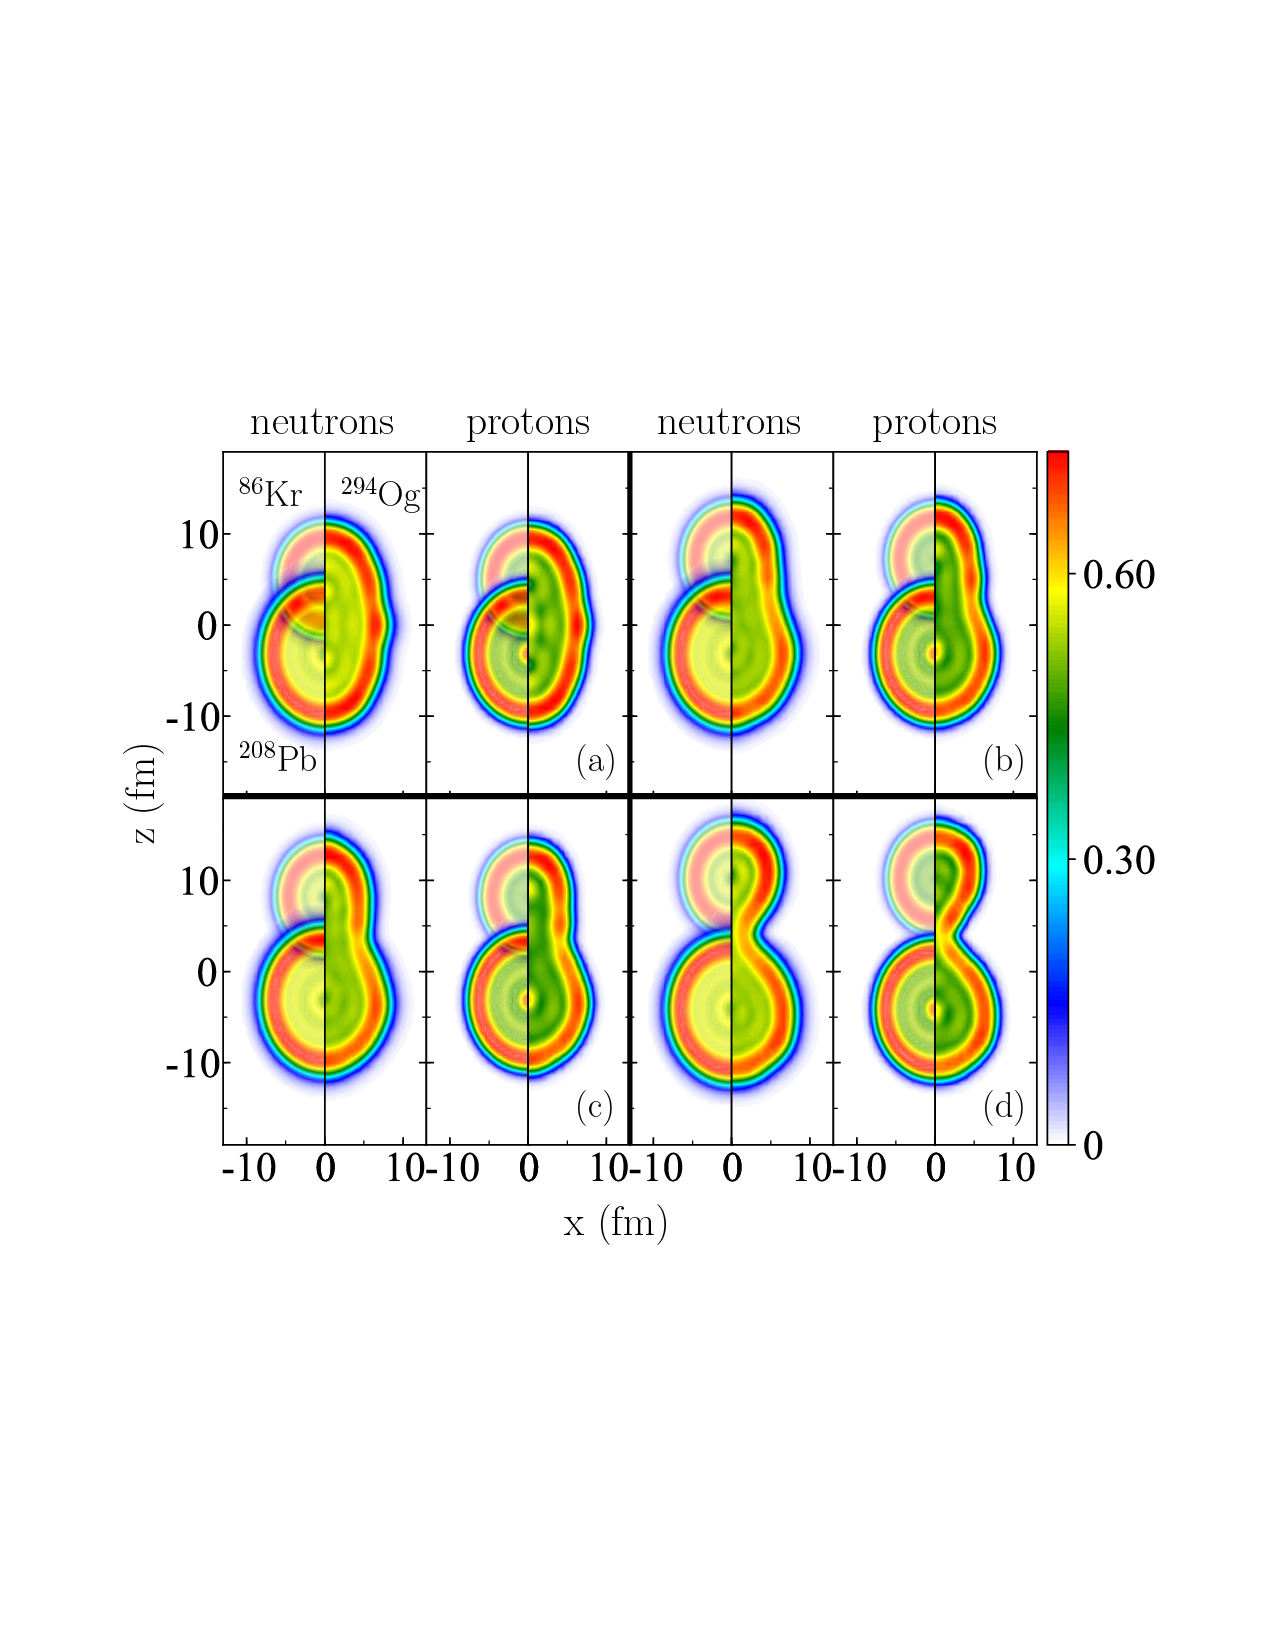
\includegraphics[width=0.9\linewidth]{TeX_files/294Og_locali}
	\caption[Nucleon localization visualization of $^{294}$Og prefragment formation.]{Nucleon localization functions for several deformed configurations of {\Og}. For comparison, localizations are also shown for the fragments {\Pb} and {\Kr} on the left side of each subplot. The configurations shown correspond to Fig. 1 from the paper, with multipole moments $(Q_{20}, Q_{30})=$ (a) (75\,b, 0); (b) (120\,b, 17\,$\mathrm{b}^\frac{3}{2}$) [${\sim}$OTL]; (c) (140\,b, 24\,$\mathrm{b}^\frac{3}{2}$); and (d) (264\,b, 60\,$\mathrm{b}^\frac{3}{2}$) [${\sim}$scission].}
	\label{fig:294oglocali}
\end{figure}

%If this is a general result, one could leverage this insight to predict fission fragments as early as the outer turning line, resulting in a major reduction in total computing time because of the reduced PES. A method which exploits this possibility is described in Appendix~\ref{append:Fragments}. % But this might have to move up, depending how the r-process calculations go


\section{Experimental search for cluster emission in $^{294}$Og}
%Perhaps the biggest uncertainty we'll see, or the biggest deviation from experiment, will be the distribution width. That's because we folded our Langevin results with a Gaussian function, the width of which was chosen rather arbitrarily to be $\sigma_A=6, \sigma_Z=4$. The values used in $^{240}$Pu were 3 and 2, but the $Q_N$ value they used to define scission was quite a bit smaller too. Since we had a much larger $Q_N$ cutoff, we needed to account for larger particle number fluctuations. But these numbers were just kind of arbitrary. I'm not too worried about this because the peak is the part that matters, and we clearly saw a peak at the cluster location.

The effort to detect cluster emission from superheavy elements is underway. However, one of the biggest challenges standing in the way of observation of cluster emission from {\Og} is the problem of statistics. There have only been 5 recorded instances of {\Og}, from the first observations in 2005~\cite{Oganessian2006} to the most recent in 2018~\cite{Brewer2018}.\footnote{In fact, there were reports as early as 2004~\cite{Oganessian2004} that fission fragments resulting from the spontaneous fission of {\Og} may have been detected, but these are unconfirmed.} To maximize the possibility of detecting spontaneous fission events as they happen, there is some discussion in the experimental community about building an ionization chamber for superheavy element research with the ability to distinguish fragments by their Z-value. This is discussed at some length in~\cite{Brewer2018}.

%``Among these SF events, there were signals correlated with incoming recoil-like signals within the time range of the {\Og} half-life. We have inspected the possible assignment of some SF events to the fission of {\Og}. In the past, as well very recently, {\Og} was considered as a system consisting of doubly magic {\Pb} and singly magic N = 50, {\Kr}. These two components are well bound stable nuclei. One can envision that an asymmetric fission of {\Og} into {\Pb} and {\Kr} fragments might be somewhat enhanced.
%
%``However, especially since the decay time of {\Og} is not sufficiently different from $^{258}$No decay, one cannot make an assignment to {\Og} activity based only on the half-life of SF events. The energy of SF events vary, since we detect sometimes only a partial energy of fission fragments. Such events are more likely to arise from the SF activity produced in a multinucleon transfer involving the Cf isotope in the target. The indistinguishability of complete-fusion from transfer reaction products provides motivation for an ionization chamber, which would have a discrimination capability for the atomic number Z, placed before the implantation Si counter. Construction and anticipated performance of such an ionization chamber based on gas electron multiplier (GEM) technology was recently discussed...'' % R-process
\chapter{Outlook}\label{chap:Outlook}

\section{Review, outlook, and perspectives}

In this chapter, it would be great to talk to everyone you know (Witek, Samuel, Jhilam, Nicolas, Michal, and so on) to get a better feel for what kinds of issues need to be addressed next. You've already got sort of a rudimentary understanding (see your Google Keep note for starters), but it might be good to get some outsider perspective. This will be especially important as you start looking for postdocs, and \textit{especially} especially if you end up looking for postdocs in nuclear theory, but not necessarily nuclear fission.

As I said in chapter \ref{chap:Intro}, ``Finally, in chapter \ref{chap:Outlook} we discuss the current state of the field, and, based on our experience, offer insights for guiding future developments in the field.''

At this stage, we have techniques to calculate half-lives and primary fragment distributions (I haven't mentioned it yet, but there is also Nicolas' method for the fragment yields that uses TD-GCM. Are there others? What about for half-lives?). Some methods (such as Walid's, TDDFT, and possibly also this GCM method) are starting to estimate fragment energetics (kinetic and excitation energies). Down the line, there are others who try to predict neutron multiplicities and goodness knows what else using Hauser-Feshbach models and such (FREYA and more). These regions are still disconnected. Of course, these methods still need major refinements in order to better reflect experimental data. Some ideas currently in the pipeline for improving the models are:

\begin{itemize}
	\item Improved EDFs (here you could mention the DME EDFs; unfortunately, introducing density-dependence has a bad effect but I forgot what it was)
	\item Improved inertia tensor (such as automatic differentiation)
	\item Better/more collective coordinates (Walid's $D, \xi$ coordinates from \cite{Younes2012}; continuity of the PES in $\infty$-dimensional space such like in David Regnier's talks and papers)
	\item Fragment identification (our localization paper, Marc Verriere's method; you might also mention that this is not an issue in TDDFT, but there you've only got one single fragment pair)
	\item Microscopic/self-consistent description for dissipation. This is the mechanism which exchanges between intrinsic and collective degrees of freedom, but we handle it in a very ad hoc way with parameters which are fitted instead of determined systematically through some theory. Solving this problem will probably help us with the energetics of fragments (TKE and E* at the same time!)
	\item Machine learning for r-process inputs (described in detail in \ref{sect:ml4rprocess})
\end{itemize}

Furthermore, there are more experimental observables that we should try to predict (refer to Andreyev's review to see what other observables can currently be measured). These include energetics (TKE and E*, for we have only begun to scratch the surface here), angular momentum, prompt neutron multiplicities (is that within the scope of these self-consistent models?), prompt neutron and gamma energy spectra spectra (getting harder; these are usually handled via statistical models; see intro to \cite{Schmidt2018} for some references), level densities?, and probably more but my mind is blanking. How to compute these in a self-consistent framework is still an open question. See also the outlook in Nicolas' review.

We definitely need a better handle on the inertia. The perturbative inertia is easy to compute, but not terribly reliable. The non-perturbative inertia can certainly do better, but as it is computed now (using finite differences) it is subject to numerical artifacts and instabilities (dependent on the level of convergence of the individual densities, the coefficient multipliers, different basis sizes) and actual physics, such as level crossings which manifest in projections from a higher-dimensional space.

UNEDF1 seems to underestimate fission barrier heights (artificial though the concept may be; the main impact is probably that lifetimes are underestimated). It also turns out to be a headache to work with, making convergence quite a challenge sometimes (any cases in particular, like for highly-deformed or heavy or octupole-deformed nuclei or something?). Better functionals might hope to better capture the physics, and one can hope they are easier to work with. % Outlook


\backmatter
% bibliography, glossary and index would go here.
\bibliography{main}
\bibliographystyle{abbrv}

\end{document}